\documentclass{article}

% packages
  % basic stuff for rendering math
  \usepackage[letterpaper, top=1in, bottom=1in, left=1in, right=1in]{geometry}
  \usepackage[utf8]{inputenc}
  \usepackage[english]{babel}
  \usepackage{amsmath} 
  \usepackage{amssymb}
  % \usepackage{amsthm}

  % extra math symbols and utilities
  \usepackage{mathtools}        % for extra stuff like \coloneqq
  \usepackage{mathrsfs}         % for extra stuff like \mathsrc{}
  \usepackage{centernot}        % for the centernot arrow 
  \usepackage{bm}               % for better boldsymbol/mathbf 
  \usepackage{enumitem}         % better control over enumerate, enumerate
  \usepackage{hyperref}         % for hypertext linking
  \usepackage{fancyvrb}          % for better verbatim environments
  \usepackage{newverbs}         % for texttt{}
  \usepackage{xcolor}           % for colored text 
  \usepackage{listings}         % to include code
  \usepackage{lstautogobble}    % helper package for code
  \usepackage{parcolumns}       % for side by side columns for two column code
  

  % page layout
  \usepackage{fancyhdr}         % for headers and footers 
  \usepackage{lastpage}         % to include last page number in footer 
  \usepackage{parskip}          % for no indentation and space between paragraphs    
  \usepackage[T1]{fontenc}      % to include \textbackslash
  \usepackage{footnote}
  \usepackage{etoolbox}

  % for custom environments
  \usepackage{tcolorbox}        % for better colored boxes in custom environments
  \tcbuselibrary{breakable}     % to allow tcolorboxes to break across pages

  % figures
  \usepackage{pgfplots}
  \pgfplotsset{compat=1.18}
  \usepackage{float}            % for [H] figure placement
  \usepackage{tikz}
  \usepackage{tikz-cd}
  \usepackage{circuitikz}
  \usetikzlibrary{arrows}
  \usetikzlibrary{positioning}
  \usetikzlibrary{calc}
  \usepackage{graphicx}
  \usepackage{caption} 
  \usepackage{subcaption}
  \captionsetup{font=small}

  % for tabular stuff 
  \usepackage{dcolumn}

  \usepackage[nottoc]{tocbibind}
  \pdfsuppresswarningpagegroup=1
  \hfuzz=5.002pt                % ignore overfull hbox badness warnings below this limit

% New and replaced operators
  \DeclareMathOperator{\Tr}{Tr}
  \DeclareMathOperator{\Sym}{Sym}
  \DeclareMathOperator{\Span}{span}
  \DeclareMathOperator{\std}{std}
  \DeclareMathOperator{\Cov}{Cov}
  \DeclareMathOperator{\Var}{Var}
  \DeclareMathOperator{\Corr}{Corr}
  \DeclareMathOperator{\pos}{pos}
  \DeclareMathOperator*{\argmin}{\arg\!\min}
  \DeclareMathOperator*{\argmax}{\arg\!\max}
  \DeclareMathOperator{\opp}{Opp}
  \DeclareMathOperator{\SRTC}{SRTC}
  \DeclareMathOperator{\SRMC}{SRMC}
  \DeclareMathOperator{\SRAC}{SRAC}
  \DeclareMathOperator{\SRAVC}{SRAVC}
  \DeclareMathOperator{\LRTC}{LRTC}
  \DeclareMathOperator{\LRMC}{LRMC}
  \DeclareMathOperator{\LRAC}{LRAC}
  \newcommand{\ket}[1]{\ensuremath{\left|#1\right\rangle}}
  \newcommand{\bra}[1]{\ensuremath{\left\langle#1\right|}}
  \newcommand{\braket}[2]{\langle #1 | #2 \rangle}
  \newcommand{\qed}{\hfill$\blacksquare$}     % I like QED squares to be black

% Custom Environments
  \newtcolorbox[auto counter, number within=section]{question}[1][]
  {
    colframe = orange!25,
    colback  = orange!10,
    coltitle = orange!20!black,  
    breakable, 
    title = \textbf{Question \thetcbcounter ~(#1)}
  }

  \newtcolorbox[auto counter, number within=section]{exercise}[1][]
  {
    colframe = teal!25,
    colback  = teal!10,
    coltitle = teal!20!black,  
    breakable, 
    title = \textbf{Exercise \thetcbcounter ~(#1)}
  }
  \newtcolorbox[auto counter, number within=section]{solution}[1][]
  {
    colframe = violet!25,
    colback  = violet!10,
    coltitle = violet!20!black,  
    breakable, 
    title = \textbf{Solution \thetcbcounter}
  }
  \newtcolorbox[auto counter, number within=section]{lemma}[1][]
  {
    colframe = red!25,
    colback  = red!10,
    coltitle = red!20!black,  
    breakable, 
    title = \textbf{Lemma \thetcbcounter ~(#1)}
  }
  \newtcolorbox[auto counter, number within=section]{theorem}[1][]
  {
    colframe = red!25,
    colback  = red!10,
    coltitle = red!20!black,  
    breakable, 
    title = \textbf{Theorem \thetcbcounter ~(#1)}
  } 
  \newtcolorbox[auto counter, number within=section]{proposition}[1][]
  {
    colframe = red!25,
    colback  = red!10,
    coltitle = red!20!black,  
    breakable, 
    title = \textbf{Proposition \thetcbcounter ~(#1)}
  } 
  \newtcolorbox[auto counter, number within=section]{corollary}[1][]
  {
    colframe = red!25,
    colback  = red!10,
    coltitle = red!20!black,  
    breakable, 
    title = \textbf{Corollary \thetcbcounter ~(#1)}
  } 
  \newtcolorbox[auto counter, number within=section]{proof}[1][]
  {
    colframe = orange!25,
    colback  = orange!10,
    coltitle = orange!20!black,  
    breakable, 
    title = \textbf{Proof. }
  } 
  \newtcolorbox[auto counter, number within=section]{definition}[1][]
  {
    colframe = yellow!25,
    colback  = yellow!10,
    coltitle = yellow!20!black,  
    breakable, 
    title = \textbf{Definition \thetcbcounter ~(#1)}
  } 
  \newtcolorbox[auto counter, number within=section]{example}[1][]
  {
    colframe = blue!25,
    colback  = blue!10,
    coltitle = blue!20!black,  
    breakable, 
    title = \textbf{Example \thetcbcounter ~(#1)}
  } 
  \newtcolorbox[auto counter, number within=section]{code}[1][]
  {
    colframe = green!25,
    colback  = green!10,
    coltitle = green!20!black,  
    breakable, 
    title = \textbf{Code \thetcbcounter ~(#1)}
  } 

  \BeforeBeginEnvironment{example}{\savenotes}
  \AfterEndEnvironment{example}{\spewnotes}
  \BeforeBeginEnvironment{lemma}{\savenotes}
  \AfterEndEnvironment{lemma}{\spewnotes}
  \BeforeBeginEnvironment{theorem}{\savenotes}
  \AfterEndEnvironment{theorem}{\spewnotes}
  \BeforeBeginEnvironment{corollary}{\savenotes}
  \AfterEndEnvironment{corollary}{\spewnotes}
  \BeforeBeginEnvironment{proposition}{\savenotes}
  \AfterEndEnvironment{proposition}{\spewnotes}
  \BeforeBeginEnvironment{definition}{\savenotes}
  \AfterEndEnvironment{definition}{\spewnotes}
  \BeforeBeginEnvironment{exercise}{\savenotes}
  \AfterEndEnvironment{exercise}{\spewnotes}
  \BeforeBeginEnvironment{proof}{\savenotes}
  \AfterEndEnvironment{proof}{\spewnotes}
  \BeforeBeginEnvironment{solution}{\savenotes}
  \AfterEndEnvironment{solution}{\spewnotes}
  \BeforeBeginEnvironment{question}{\savenotes}
  \AfterEndEnvironment{question}{\spewnotes}
  \BeforeBeginEnvironment{code}{\savenotes}
  \AfterEndEnvironment{code}{\spewnotes}

  \definecolor{dkgreen}{rgb}{0,0.6,0}
  \definecolor{gray}{rgb}{0.5,0.5,0.5}
  \definecolor{mauve}{rgb}{0.58,0,0.82}
  \definecolor{lightgray}{gray}{0.93}

  % default options for listings (for code)
  \lstset{
    autogobble,
    frame=ltbr,
    language=C,                           % the language of the code
    aboveskip=3mm,
    belowskip=3mm,
    showstringspaces=false,
    columns=fullflexible,
    keepspaces=true,
    basicstyle={\small\ttfamily},
    numbers=left,
    firstnumber=1,                        % start line number at 1
    numberstyle=\tiny\color{gray},
    keywordstyle=\color{blue},
    commentstyle=\color{dkgreen},
    stringstyle=\color{mauve},
    backgroundcolor=\color{lightgray}, 
    breaklines=true,                      % break lines
    breakatwhitespace=true,
    tabsize=3, 
    xleftmargin=2em, 
    framexleftmargin=1.5em, 
    stepnumber=1
  }

% Page style
  \pagestyle{fancy}
  \fancyhead[L]{Microeconomics}
  \fancyhead[C]{Muchang Bahng}
  \fancyhead[R]{Summer 2024} 
  \fancyfoot[C]{\thepage / \pageref{LastPage}}
  \renewcommand{\footrulewidth}{0.4pt}          % the footer line should be 0.4pt wide
  \renewcommand{\thispagestyle}[1]{}  % needed to include headers in title page

\begin{document}

\title{Microeconomics}
\author{Muchang Bahng}
\date{Summer 2024}

\maketitle
\tableofcontents
\pagebreak

\section{General Principles of Markets} 

  \subsection{Supply and Demand: Definitions}

    We introduce the foundational concepts of classical economics: supply and demand. Even though these definitions have much similarities with how they are used in colloquial English language, there are subtle differences and difficulties in formalizing their definitions. Therefore, we will consider the following definitions quite loosely:
    \begin{enumerate}
      \item The \textbf{demand} of a good $G$ is known as how much consumers are willing to buy that good $G$, represented as the total amount of units that consumers willing to buy. It is a sign of how needed or wanted that good is. e.g. consumers are willing to buy 1 billion toothbrushes in America.
      \item The \textbf{supply} of a good $G$ is known as how much producers are willing to sell that good $G$, represented as the total amount of units that producers are willing (to make and) to sell. It is a sign of how much of the good is available. e.g. producers are willing to sell 100,000 tables per year in the state of California.
    \end{enumerate}

  \subsection{Marginal Value \& Marginal Cost Curves}

    Before we go any further, observe some basic facts. Whenever a consumer buys a good $G$ for price $P$, by rationality they are buying it because they believe that the value they gain by obtaining a unit of $G$ is greater than that of the price $P$. This is indeed the case since, by the \textbf{law of diminishing returns}, for each successive unit of $G$ the marginal value of one additional unit of $G$ decreases, until there is a point where buying another unit is not worth paying $P$.
    \begin{center}
      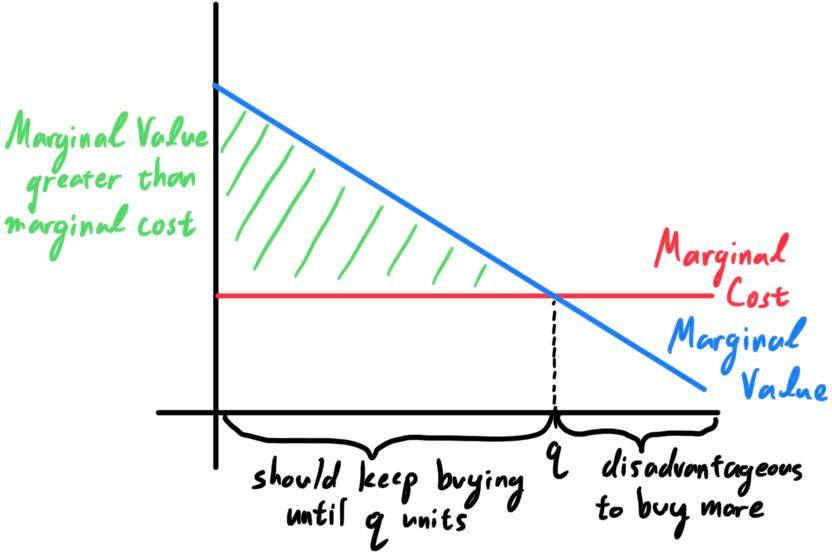
\includegraphics[width=0.9\textwidth]{img/Marginal_Value.jpg}
    \end{center}

    Additionally, when a supplier sells a good $G$ for price $P$, by rationality they are selling it because they believe that the value they gain by producing and selling a unit of $G$ is greater than that of the price $P$. For some reason I can't find a deeper reason for this than the qualitative description: a higher price will induce producers to supply a higher quantity to the market to maximize profits. I'm sure there is some reason concerning the marginal supply curve, but I have yet to figure this out for some time.

  \subsection{Supply Curves \& Demand Curves}

    To formalize these concepts mathematically, we now introduce the demand and supply functions, with a simple property for each. The \textbf{demand function} $D_G$ of a certain good $G$ maps a certain price $P$ representing the price that consumers will buy a unit of $G$, and outputs the \textbf{demand} of $G$ in a quantity of $Q$ units.
    \begin{equation}
      D: P \longrightarrow Q
    \end{equation}

    Due to the \textbf{law of demand}, this demand function is monotonically decreasing, i.e. the demand is inversely proportional to the price. We can roughly see why because an increase in the price that consumers will buy a unit of $G$ will cause them to buy less, due to an overall smaller marginal value.
    \begin{center}
      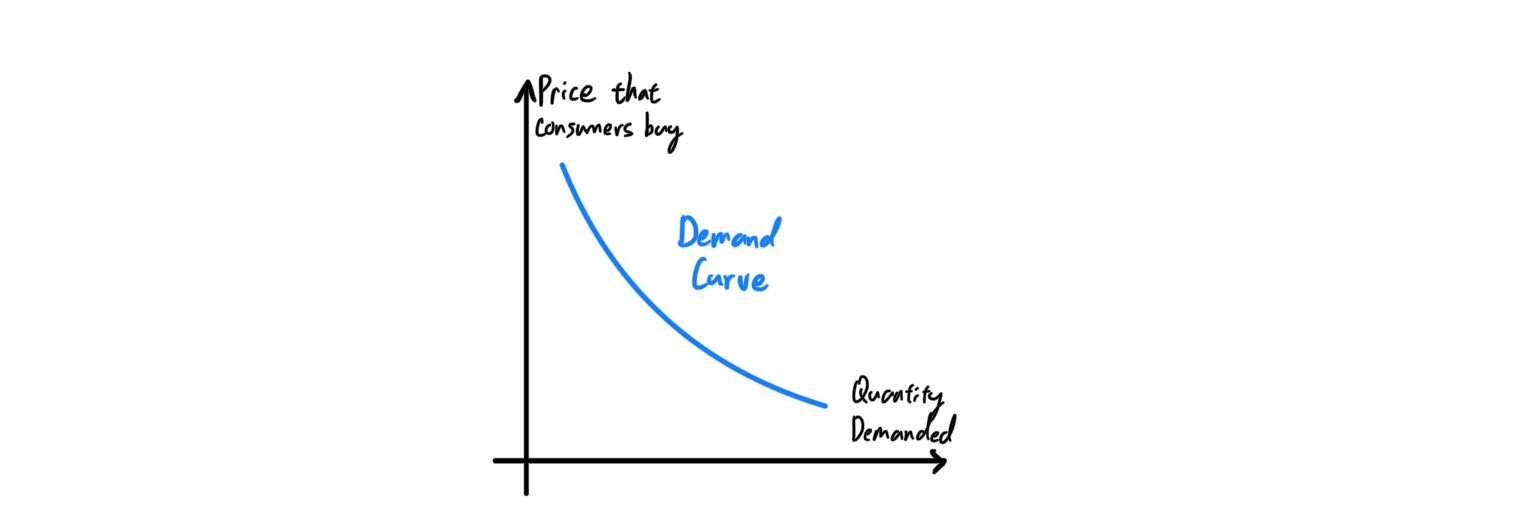
\includegraphics[width=0.9\textwidth]{img/Demand_Curve.jpg}
    \end{center}

    The \textbf{supply function} $S_G$ of a certain good $G$ maps a certain price $P$ representing the price that producers will sell a unit of $G$, and outputs the \textbf{supply} of $G$ in a quantity of $Q$ units.

    \begin{equation}
      S: P \longrightarrow Q
    \end{equation}
    Due to the \textbf{law of supply}, this supply function is monotonically increasing, i.e. the supply is directly proportional to the price. We can roughly see why because an increase in the price that producers will sell a unit of $G$ will cause them to sell more, due to an overall greater profit margin.

    \begin{center}
      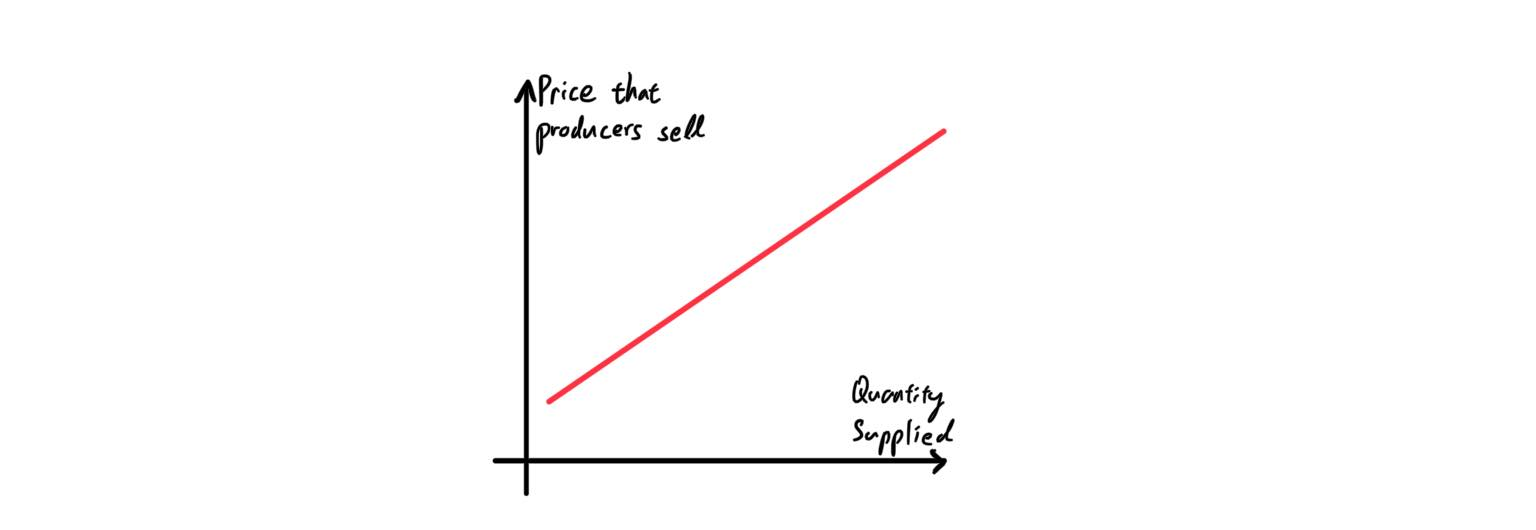
\includegraphics[width=0.9\textwidth]{img/Supply_Curve.jpg}
    \end{center}
    Note that this notation for the domains and codomains of both $D$ and $S$ may be misinterpreted to represent the same quantity, but this is not the case. The domain $P$ of $D$ is the price in which the consumers buy, while the domain $P$ of $S$ is the price in which the suppliers sell. The codomain $Q$ of $D$ is the quantity demanded, while the codomain $Q$ of $S$ is the quantity supplied.

  \subsection{Supply \& Demand Curves Together and Equilibrium}

    In a market, we have both the sellers and the buyers, so it would make sense to put both curves in the same graph.
    \begin{center}
      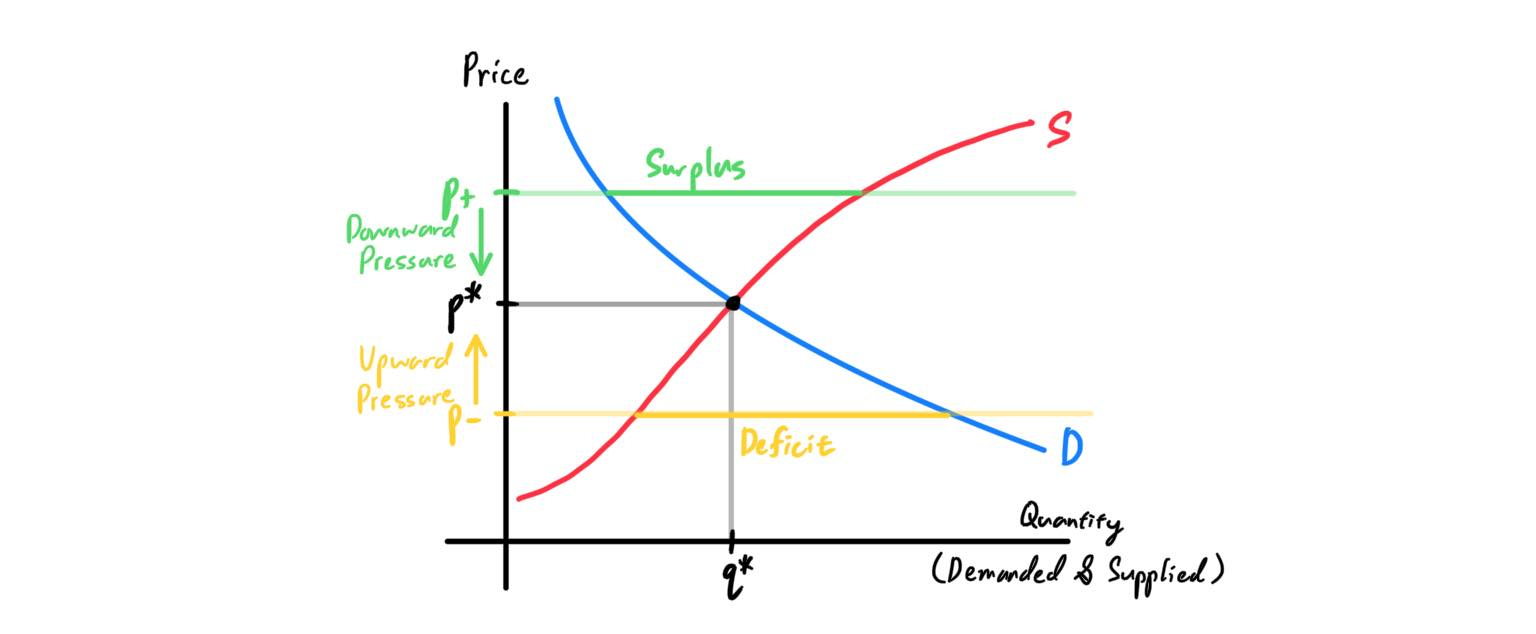
\includegraphics[width=0.9\textwidth]{img/Supply_and_Demand.jpg}
    \end{center}
    Now using both the \textbf{laws of supply and demand}, let us describe how market forces will act on the trading of goods.
    \begin{enumerate}
      \item Assume that the price of good $G$ is $p_{-} < p$. Then, there will be a deficit of $G$. Consumers will compete to buy these, which will put upwards pressure on the price.
      \item Assume that the price of good $G$ is $p_{+} > p$. Then, there will be a surplus of $G$. Producers will optimize their prices to sell, which will put downwards pressure on the price.
    \end{enumerate}
    These \textbf{movements in the supply and demand curve} leads to the price and quantity demanded/supplied converging onto an equilibrium point, labeled with $p^\ast$ and $q^\ast$, respectively.

  \subsection{Shifts in Supply and Demand}

    An \textbf{increase in demand} simply means that consumers are willing to pay more for the same quantity of a good $G$ (note that this is equivalent to saying that consumers are willing to buy less of $G$ for the same price). This results in an up-rightward shift in the demand curve.
    \begin{center}
      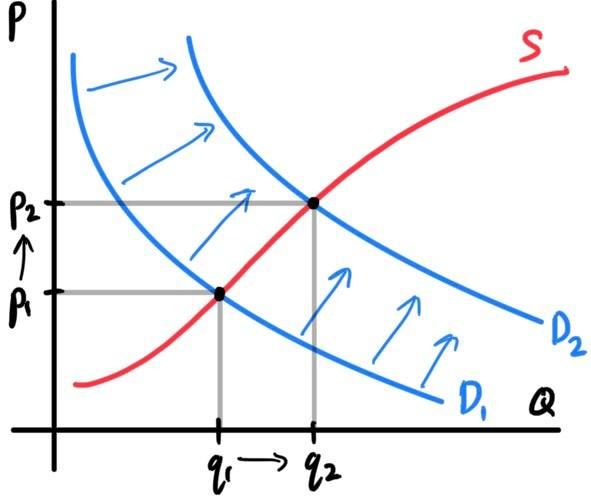
\includegraphics[width=0.5\textwidth]{img/Increase_in_Demand.jpg}
    \end{center}
    A change in demand describes the case when the consumers of a given good or service alter their means of consumption. Here are some examples of when demand changes (note that this shift in demand is different from a change in\textit{quantity} demanded):
    \begin{enumerate}
    \item A shift in population demographic could require the use for more wheelchairs and canes.
    \item A product mentioned in a popular Netflix show would increase demand for said product.
    \end{enumerate}
    An \textbf{increase in supply} simply means that producers are willing to sell more at the same price $p$. This results in an up-leftward shift in the supply curve.
    \begin{center}
      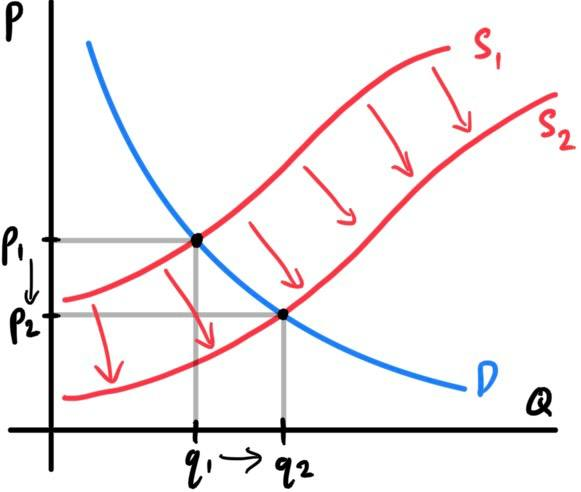
\includegraphics[width=0.5\textwidth]{img/Increase_in_Supply.jpg}
    \end{center}
    A change in supply describes the case when the suppliers of a given good or service alter production or output. Here are some examples of when supply changes (note that this shift in supply is different from a change in\textit{quantity} supplied):
    \begin{enumerate}
    \item The price of raw materials can increase, resulting in lower prices.
    \item War against Russia results in sanctions on oil imports into the U.S., decreasing the supply.
    \end{enumerate}

  \subsection{Market in Perfect Equilibrium}

    Let us construct a market from scratch, and with it the general principles that they follow. Assume that civilization has evolved enough to acquire specialization of labour. Let us have three entities, labeled $E_1, E_2, E_3$ with the following properties:
    \begin{enumerate}
      \item Annually, $E_1$ produces $1000$ units of good $G_1$. $E_1$ has an annual requirement of $100$ units of $G_2$ and $0$ units of $G_3$.
      \item Annually, $E_2$ produces $800$ units of good $G_2$. $E_2$ has an annual requirement of $300$ units of $G_1$ and $400$ units of $G_3$.
      \item Annually, $E_3$ produces $900$ units of good $G_3$. $E_3$ has an annual requirement of $200$ units of $G_1$ and $500$ units of $G_2$.
    \end{enumerate}
    Through \textbf{trade}, these entities can take advantage of their \textbf{comparative advantages} for greater efficiency.
    \begin{center}
      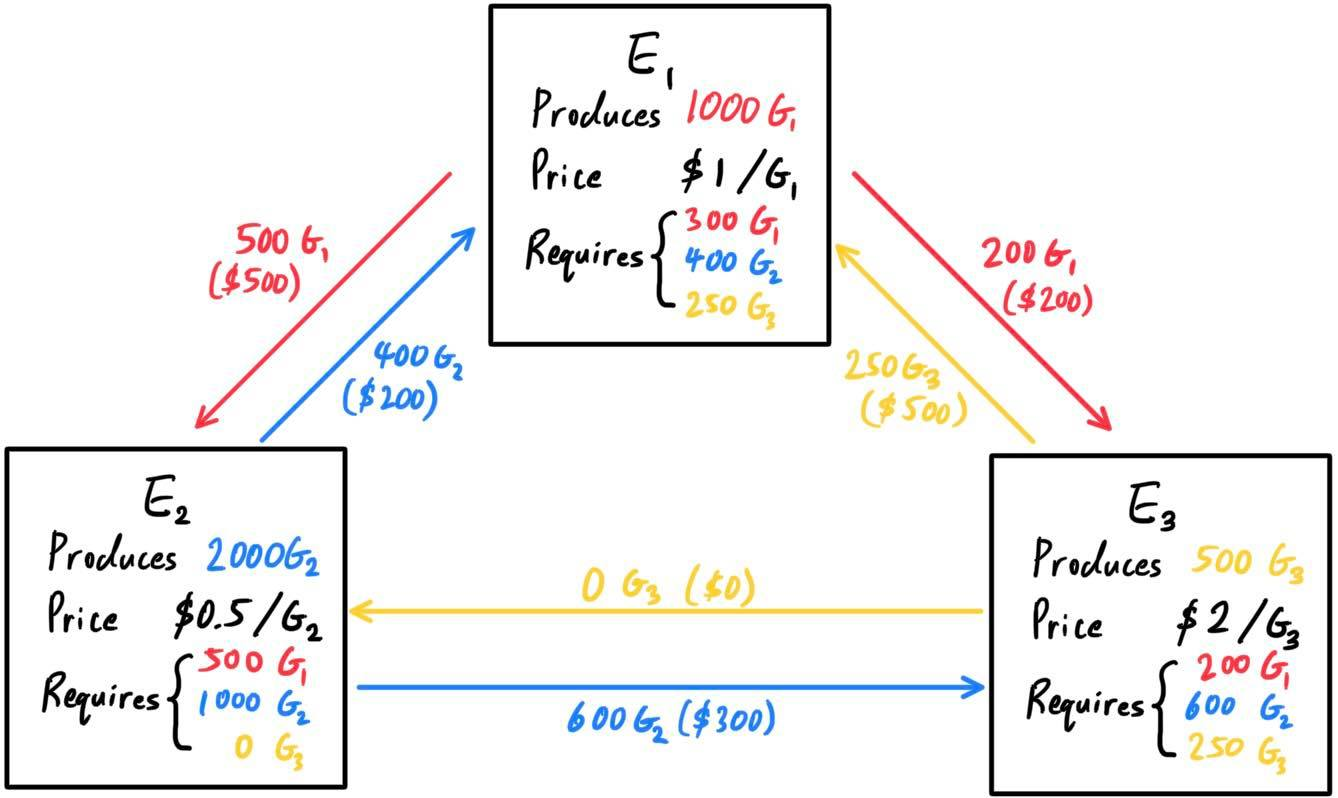
\includegraphics[width=0.9\textwidth]{img/Initial_Trade.jpg}
    \end{center}
    If we look at the market supply and market demand curves for each of the three goods in this 3-entity economy, we will see:
    \begin{center}
      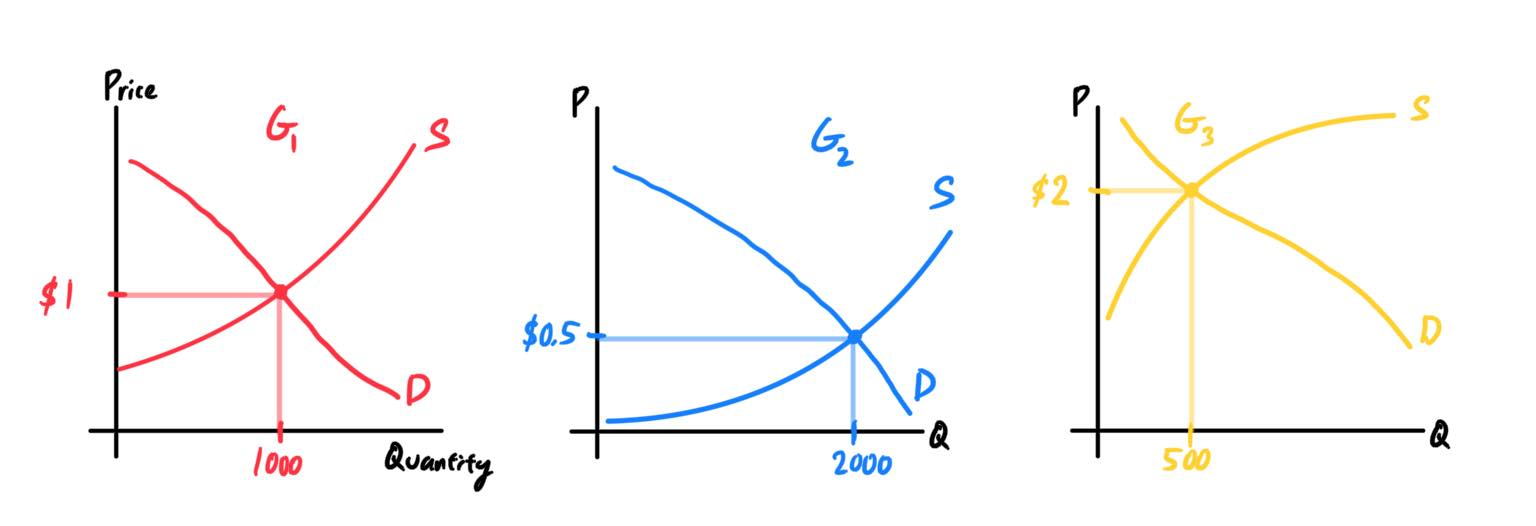
\includegraphics[width=0.9\textwidth]{img/Supply_Demand_Curves_of_3_Goods.jpg}
    \end{center}
    Note that these are \textbf{market curves} which represents the sum of all the supplies and demands of the individuals within a market. In other words, the \textbf{demand of good $G_1$ (of a market)} is the sum of the demands of all buyers in the market. The \textbf{supply of good $G_1$ (in a market)} is the sum of the supplies of all sellers in the market. But this concept of the market curve is too abstract. What does it actually mean to talk about the supply and demand of a good within a market? Let's consider a bigger market with $n$ entities, $E_1, E_2, \ldots, E_n$, and just one good $G_1$. Now, note that we make a few assumptions:
    \begin{enumerate}
      \item All entities $E_i$ have perfect communication with each other. That is, everybody know what everybody else is buying and selling for their respective prices.
      \item The price at which a unit is \textit{sold} is the same for all suppliers. If two entities $E_1$ and $E_2$ sold a unit of good $G$ at different prices, by assumption $1$ all possible consumers would go to whoever is selling at the lower price, pressuring the other to lower its price to match.
      \item The price at which a unit is \textit{bought} is the same for all consumers. If two entities $E_1$ and $E_2$ want to buy a unit of good $G$ at different prices, by assumption 1 all possible suppliers would go to whoever is buying at the higher price, pressuring the other to raise its bid to match.
    \end{enumerate}
    Now, good $G$, assuming it is liquid and on a large scale, is circulating countless times among entities as $E_i$ sells to $E_j$. But a \textbf{transaction} can only happen from $E_i$ to $E_j$ if it meets two conditions:
    \begin{enumerate}
      \item $E_j$ is willing to buy $G$: that is, the \textbf{marginal value} of an additional unit of $G_1$ is greater than the price.
      \item $E_i$ is willing to sell $G$: that is, the \textbf{marginal cost} of an additional unit of $G_1$ is less than the price.
    \end{enumerate}
    These two assumptions can be nicely summarized as
    \begin{equation}
      \text{Marginal Cost of Producing } < \text{ Price of Selling } = \text{ Price of Buying } < \text{ Marginal Value of Buying}
    \end{equation}
    If this happens, we can assume that $E_i$ and $E_j$ will automatically trade. Therefore, we can see that:
    \begin{enumerate}
      \item The (market) supply of $G_1$ is $1000$ units, since that is how much all the producers (just $E_1$ in this case) are willing to produce until its marginal costs of producing is greater than the price at which they sell. More specifically, since $E_1$ also consmues $300$ units, the supply in the \textbf{exchange market} between the three entities is $700$ units of $G_1$.
      \item The (market) demand of $G_1$ is also $1000$ units, since that is how much all the consumers ($E_1, E_2, E_3$) are willing to produce until its marginal value of buying is less than the price at which they buy. More specificaly, since $E_1$ also consumes $300$ units, the demand in the exchange market between the three entities is also $700$ units of $G_1$.
    \end{enumerate}

  \subsection{Fluctuations in Market Supply and Its Effects}

    If production is consistent, all is well and everyone lives happily ever after in this state of equilibrium. But with the actual fluctations that occurs in the real world (affected by climate, labor, war, disease, etc.), without loss of generality, $E_1$ may either underproduce or overproduce its optimal amount of $1000$ units of $G_1$.

    We will first introduce a \textit{wrong} interpretation that I have fallen for many times. The following below is a naive way of interpreting situations when there are fluctuations in supply and demand, which ignores all the concepts that was introduced previously.

    \begin{enumerate}
      \item When $E_1$ produces $1200$ units of $G_1$ and uses $300$ units, then there are now $900$ units of $G_1$ that is left for sale in the market, so the market supply is $900$ units. The demand is still $700$ since the needs of entities $E_2$ and $E_3$ haven't changed. Therefore, this surplus of $200$ units is wasted and not bought because $E_2$ and $E_3$ do not need it anymore. It is as good as dead.
      \item When $E_1$ produces $800$ units of $G_1$ and uses $300$ units, then there are now $500$ units of $G_1$ that is left for sale in the market, so the market supply is $500$ units. The demand is still $700$ since the needs of entities $E_2$ and $E_3$ haven't changed. This shortage of $200$ units will cause distress, but nothing can be done about it within this economy.
    \end{enumerate}

    These cases represents a \textit{change in supply}. Note that this does \textit{not} mean a change in quantity supplied, since quantity supplied would be caused by a change in price (remember, $S$ maps price to quantities). Remember our laws that a change in supply will have an efffect on the price (upwards or downwards pressure).

    \begin{enumerate}
      \item If the supply of good $G_1$ changes from $1000$ units to $1200$ units, then the supply curve will increase, causing the equilibrium price to fall to $0.8$ dollars at point $eq_2$ and the quantity demanded to increase.
      \begin{center}
        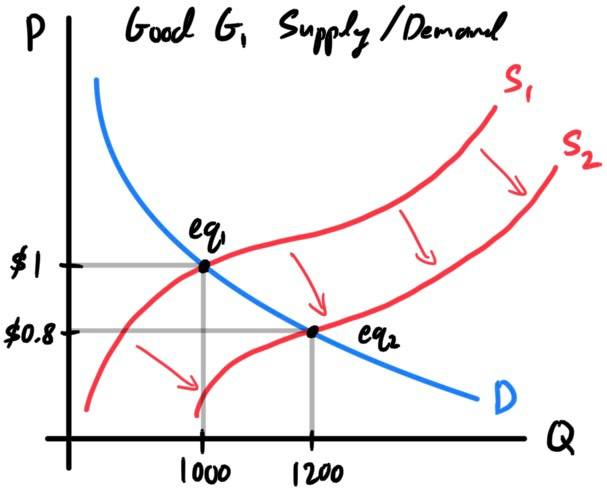
\includegraphics[width=0.5\textwidth]{img/Supply_Inc.jpg}
      \end{center}
      Note that since supply is a continuous process this change should happen continuously, but if for some reason this change in supply happens extremely fast, or if there is a restriction on the price to be 1 dollar, then the price/quantity supplied data will be at point $k$. In this moment, with the price fixed at $1$ dollar, the quantity demanded would naturally be $1000$, while the actual supply would be $1200$, leading to a surplus of $200$. Eventually, the price will drop down from $k$ to the equilibrium point $eq_2$.
      \begin{center}
        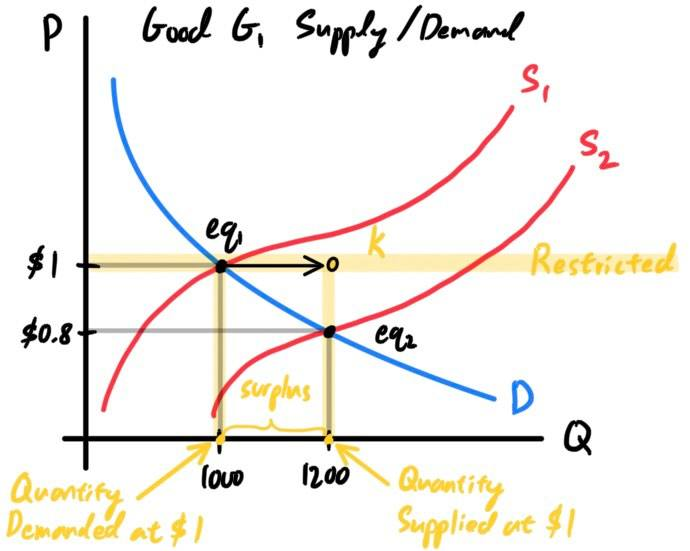
\includegraphics[width=0.5\textwidth]{img/Supply_Inc_2.jpg}
      \end{center}

      \item If the supply of good $G_1$ changes from $1000$ units to $800$ units, then the supply curve will decrease, causing the equilibrium price to rise to $1.2$ dollars at the point $eq_2$ and the quantity demanded to decrease.
      \begin{center}
        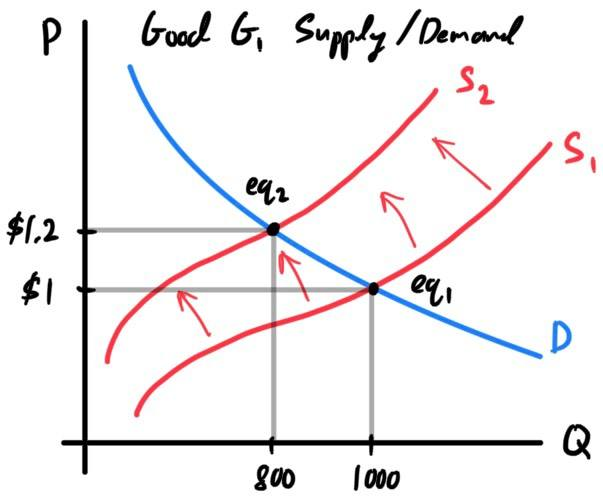
\includegraphics[width=0.5\textwidth]{img/Supply_Dec.jpg}
      \end{center}
      Again, this should happen continuously, but if for some reason this change in supply happens extremely fast, or if there is a restriction on the price to be 1 dollar, then the price/quantity supplied data will be at $k$. In this moment, with the price fixed at 1 dollar, the quantity demanded would be $1000$ while the actual supply would be $800$, leading to a surplus of $200$. Eventually, the price will rise from $k$ to the equilibrium point at $eq_2$.
      \begin{center}
        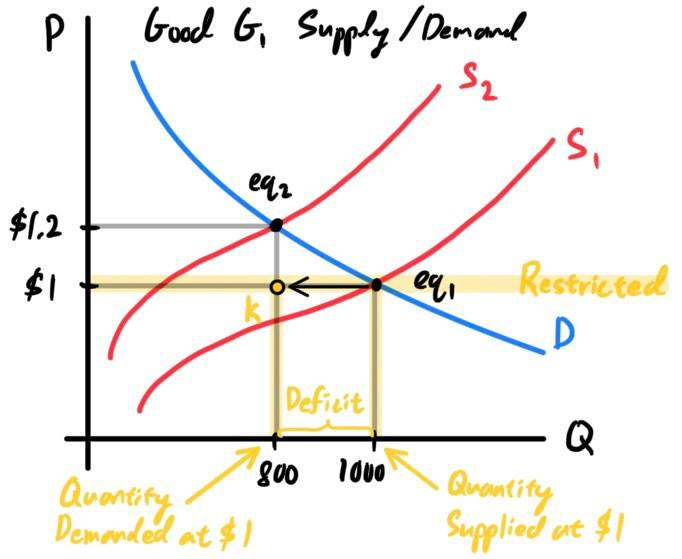
\includegraphics[width=0.5\textwidth]{img/Supply_Dec_2.jpg}
      \end{center}
    \end{enumerate}
    Technically, I guess it is possible to model with sufficient accuracy the smooth change in the supply as a bunch of infinitesimal changes that I have described happening in a row. This is what Adam Smith refers to as the \textbf{invisible hand}.

    Finally, note that in this context (and in most contexts), the supply of a good really means \textit{the supply of a good that is available to trade within the market}. Goods that are not in some market do not go by these laws of supply and demand. Examples include
    \begin{enumerate}
      \item National oil reserves, which are not bought or sold and therefore do not contribute to the supply of an entity (in this case, a nation).
      \item Privately held stocks (RSU), which do not circulate in the market since they are held for long periods of time and are not sold.
    \end{enumerate}

  \subsection{Elasticities}

    In general, \textbf{elasticity} refers to the rate at which a value is affected by a change in another value. It is a mathematical way of describing how the supply and demand curves are "shaped" (i.e. are they steep? flat? curved? etc.). There are two types of elasticities:
    \begin{enumerate}
      \item The \textbf{price-elasticity of demand} refers to how sensitive the quantity demanded is to a change in price.
      \begin{enumerate}
        \item If a price change of $G$ leads to a greater change in quantity demanded, then $G$ is said to be elastic (demand curve becomes flatter). A perfectly elastic demand curve is flat.
        \item If a price change of $G$ leads to a smaller change in quantity demanded, then $G$ is said to be inelastic (demand curve becomes steeper). A perfectly inelastic demand curve is vertical.
      \end{enumerate}

      \item The \textbf{price-elasticity of supply} refers to how sensitive the quantity supplied is to a change in price.
      \begin{enumerate}
        \item If a price change of $G$ leads to a greater change in quantity supplied, then $G$ is said to be elastic (supply curve becomes flatter). A perfectly elastic supply curve is flat.
        \item If a price change of $G$ leads to a smaller change in quantity supplied, then $G$ is said to be inelastic (supply curve becomes steeper). A perfectly inelastic supply curve is vertical.
      \end{enumerate}

    \end{enumerate}
    There is a precise mathematical formulation for elasticity, but we will not go over them here. Just note a few examples:
    \begin{enumerate}
      \item The elasticity of demand of insulin shots is low, since it is a necessary product, a consumer staple. A change in price will not cause consumers who need them to stop buying them.
      \item The elasticity of demand of computers is high, since it is not a necessary product; it is a discretionary product. A change in price will cause many consumers to stop buying them.
      \item The elasticity of supply of coffee is high, since a rise in price will cause suppliers to produce more of them.
      \item The elasticity of supply of grapes is low, since harvest is once a year, so a rise or fall in price will not change much of how they are produced.
    \end{enumerate}

\section{Supply and Demand}

  Note that the models inherently deal with discrete values, but for the sake of simplicity, we represent them as a continuum. This results in two (equivalent) interpretations of the word \textbf{marginal}: 
  \begin{enumerate}
    \item Discrete case: marginal value can refer to the additional value gotten from the next unit. 
    \item Continuous case: marginal value can refer to the derivative of the total value. 
  \end{enumerate}
  Equivalent scenarios between both cases are: 
  \begin{enumerate}
    \item Additional value of the next unit is positive but not as positive as the value gotten from the current unit $\iff$ the marginal value has positive values, but is sloping down
    \item Additional value of the next unit is positive and is more positive than the value gotten from the current unit $\iff$ the marginal value has positive values and is sloping up
    \begin{center}
      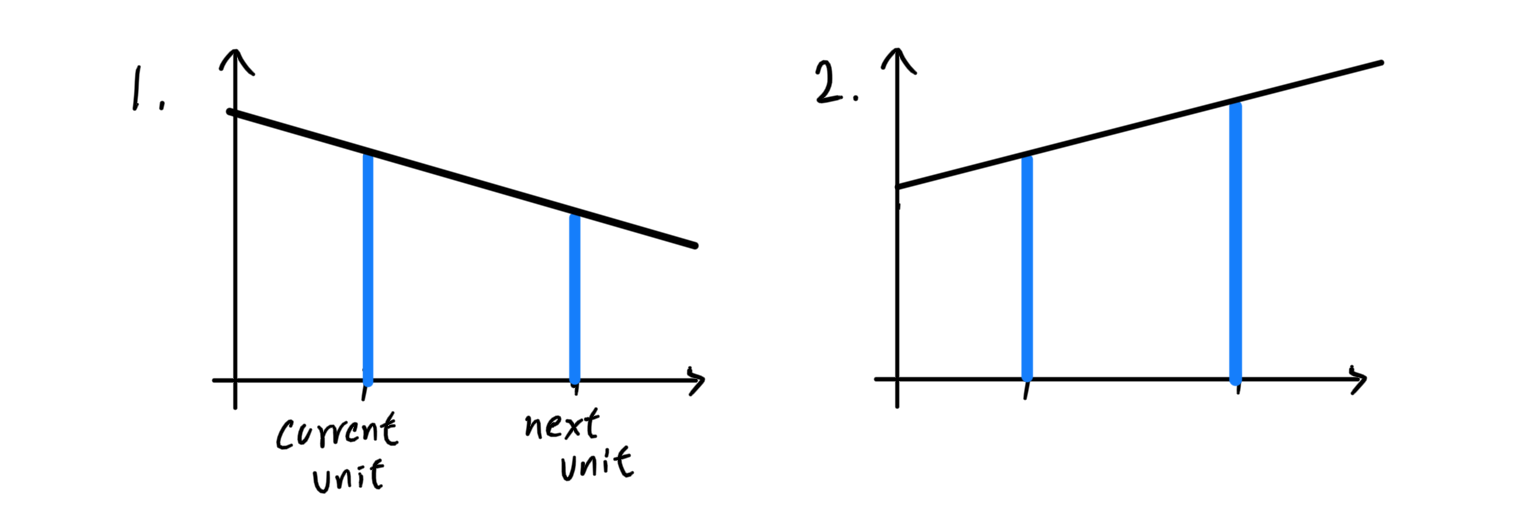
\includegraphics[scale=0.25]{img/12.PNG}
    \end{center}
    \item Additional value of the next unit is negative but not as negative as the value gotten from the current unit $\iff$ the marginal value has negative values but sloping up
    \item Additional value of the next unit is negative and is more negative than the value gotten from the current unit $\iff$ the marginal value has negative values and is sloping down
    \begin{center}
      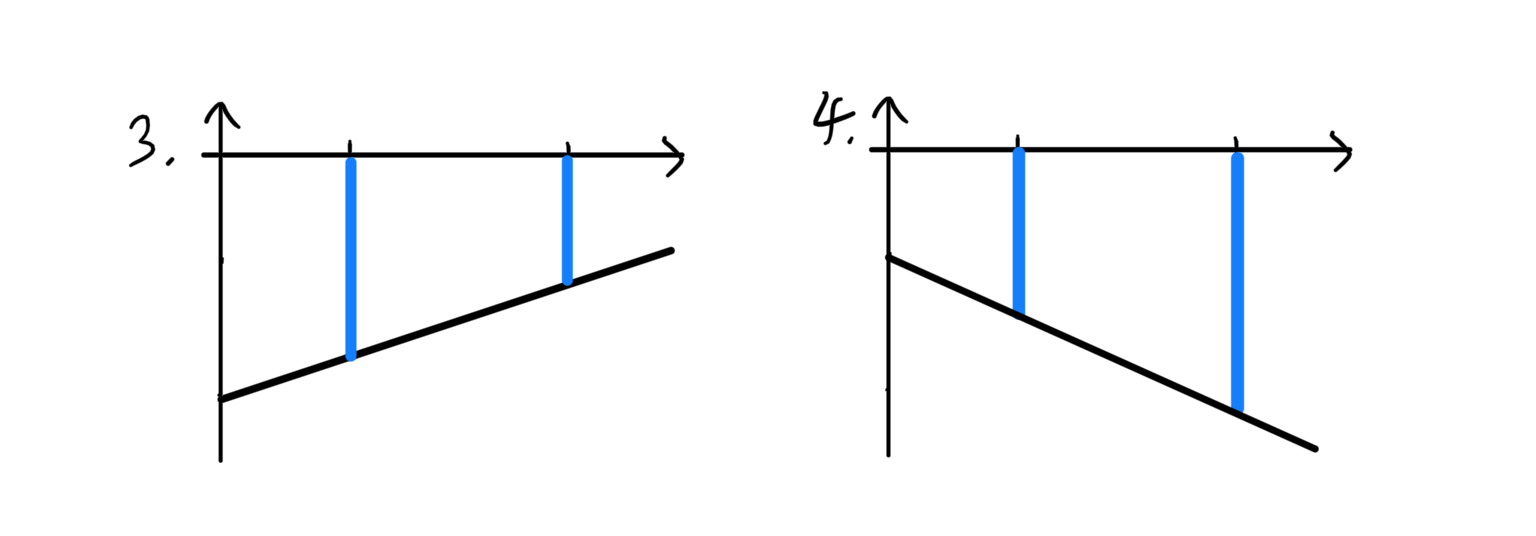
\includegraphics[scale=0.25]{img/34.PNG}
    \end{center}
  \end{enumerate}

  \subsection{Marginal Value Curves, Demand Curves, and Consumer Surplus}

    Given a consumer and a certain good $\mathfrak{g}$, we can identify 2 values: 
    \begin{enumerate}
      \item The individual's willingness to pay for an additional unit of that good (which can change over time). This can be interpreted as the consumer's "personal value" of $\mathfrak{g}$, which can be monetized to the maximum price that the individual is willing to pay for $\mathfrak{g}$. 
      \item The actual price of $\mathfrak{g}$ (which is assumed to be constant)
    \end{enumerate}
    For example, Jason loves bananas and is willing to pay up to \$10 for a banana (personal value) and the store sells them at a price of \$1 per banana. 

    We present a critical (yet not an unreasonable) assumption. 

    \begin{definition}[Principle of Diminishing Marginal Value]
      Even though there are exceptions, the marginal value for most goods diminish. That is, the additional value of additional units of $\mathfrak{g}$ decreases. 
    \end{definition}

    \begin{example}
      Jason's is willing to buy \$10 of his first banana, but is willing to pay only \$8 for the second banana, \$6 for the third, \$4 for the fourth, \$2 for the fifth, and \$0 for the sixth. This means that after five bananas, he is indifferent to getting an additional banana. 
    \end{example}

    \begin{definition}[Total Value Curve]
      We can plot the total (monetized) value that each good brings a consumer by graphing the \textbf{total value curve}. This can be defined by the function $v_T$
      \[v_T: \big( \text{quantity } q \text{ of } \mathfrak{g}\big) \mapsto \big(\text{total monetized value that buying } q \text{ units brings} \big)\]
      \begin{center}
          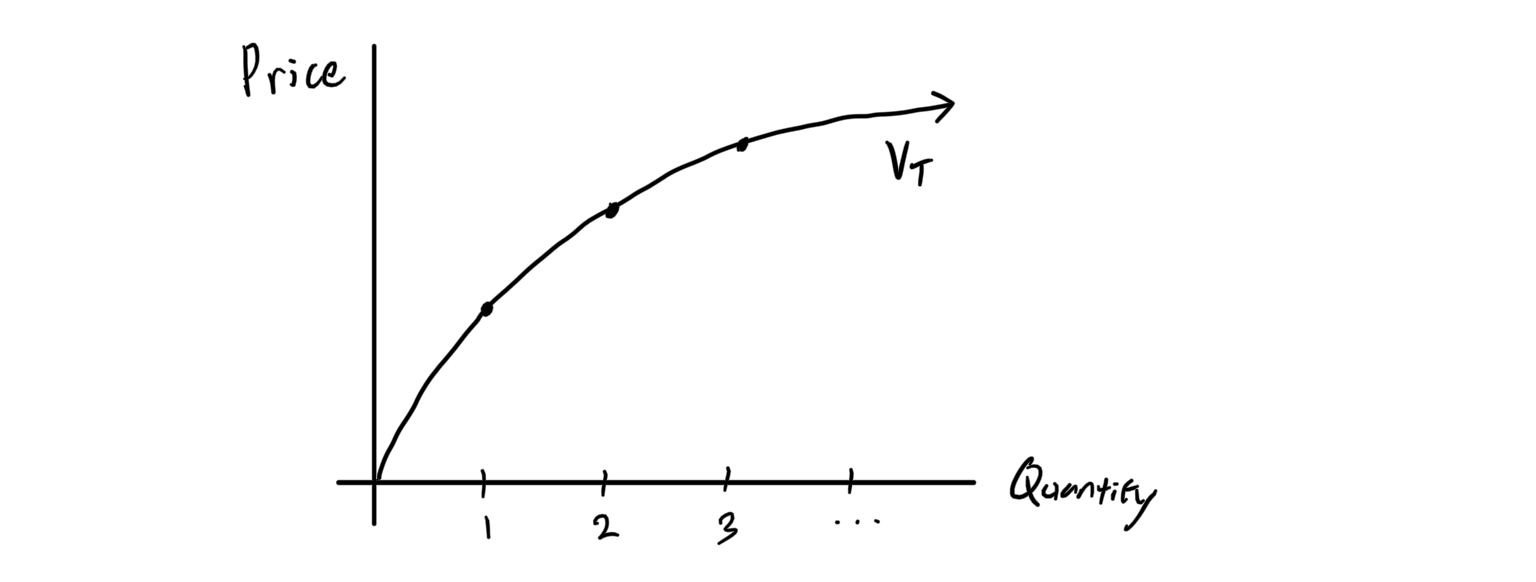
\includegraphics[scale=0.25]{img/Total_Value_Curve.PNG}
      \end{center}
      When we have 0 units of the good, our total value is 0 since we have nothing. Having 1 unit of the good increases our total value. Having an additional unit of the good increases our total value again, but not as much as the first unit did. The same goes for the third value. We can mathematically describe this by saying that the graph of $v_T$ is \textit{convex}, or \textit{concave down}. 
    \end{definition}

    Conventionally, we work a lot more with marginal value curves. 

    \begin{definition}[Marginal Value Curve]
      The \textbf{marginal value curve}, denoted $v_M$, is the derivative of the total value curve. 
      \[v_M = \frac{d v_T}{d q}\]
      as the name suggests, 
      \[v_M: \big( \text{quantity } q \text{ of } \mathfrak{g}\big) \mapsto \big(\text{marginal value of next unit} \big)\]
      By the principal of diminishing marginal value, $v_M$ must be monotonically decreasing. 
      \begin{center}
          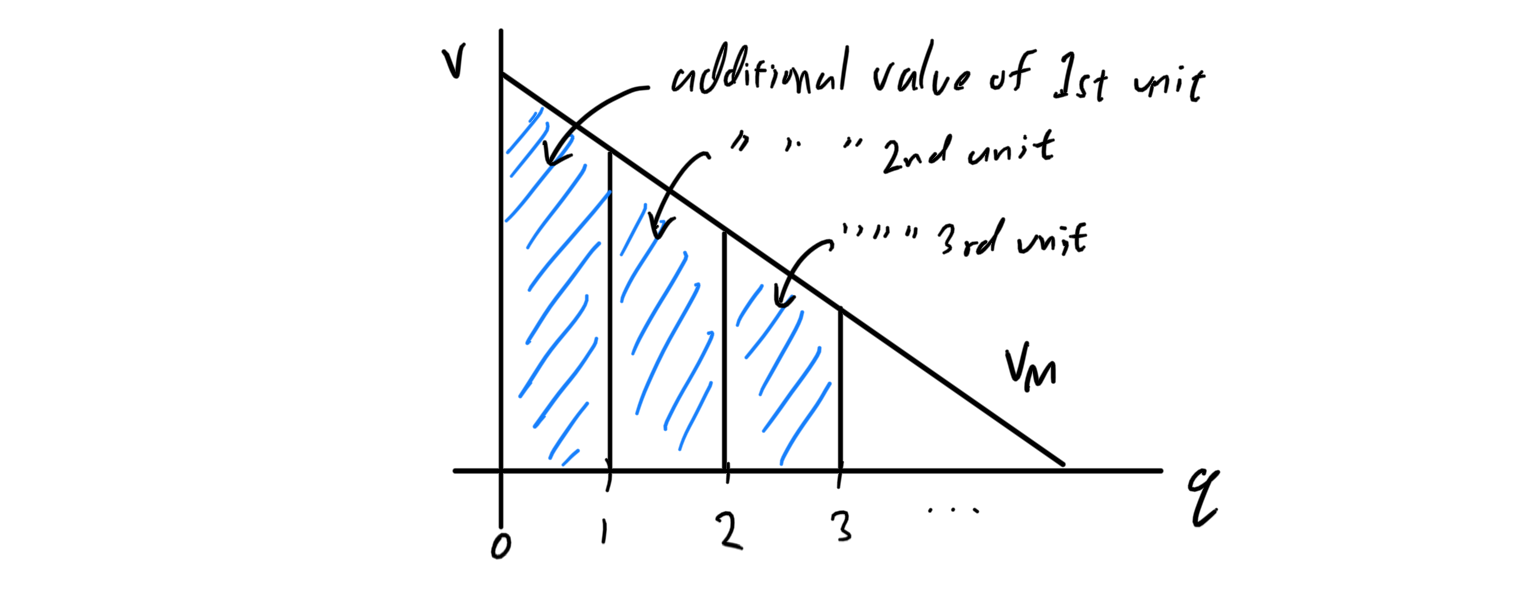
\includegraphics[scale=0.25]{img/Marginal_Value_Curve.PNG}
      \end{center}
      Furthermore, we can see that the area under the curve represents the additional value that each unit has added. That is, each "bar" represents the value of that additional unit. More formally, 
      \[\int_{i-1}^{i} v_M (q) dq\]
      represents the value added by the $i$th unit of good, and 
      \[v_T (q) = \int_0^q v_M (x) \,dx\]
    \end{definition}

    While we get a certain (monetized) marginal value from buying one more unit of $\mathfrak{g}$, we have assumed up to now that we get these for free. This isn't the case, since a unit of a good has a certain price that we pay for. In addition to the marginal value curve, we can graph the \textbf{marginal cost curve}, which basically represents the cost of an additional unit of $\mathfrak{g}$ (assumed to be constant). Let's call this value $p$, which stands for "price." 

    \begin{definition}[Consumer Surplus]
      We see that as long as the marginal value is greater than the marginal cost, the consumer would get a net profit. This profit is called the \textbf{consumer surplus}. One can see that the consumer surplus is greatest on the first purchase of $\mathfrak{g}$ and then decreases to $0$ and negative values with enough purchases. Mathematically, it is defined 
      \[CS_{q} = v_M (q) - p\]
      Another definition of consumer surplus is the \textit{maximum profit} a consumer could make, given the marginal value and cost. This would be found by summing up all of the individual profits until the point $q_0$, which represents the point where the marginal profit is equal to the marginal cost. Mathematically, it is defined 
      \[CS = \int_{0}^{q_0} v_M (q) - p \,dq\]
      \begin{center}
        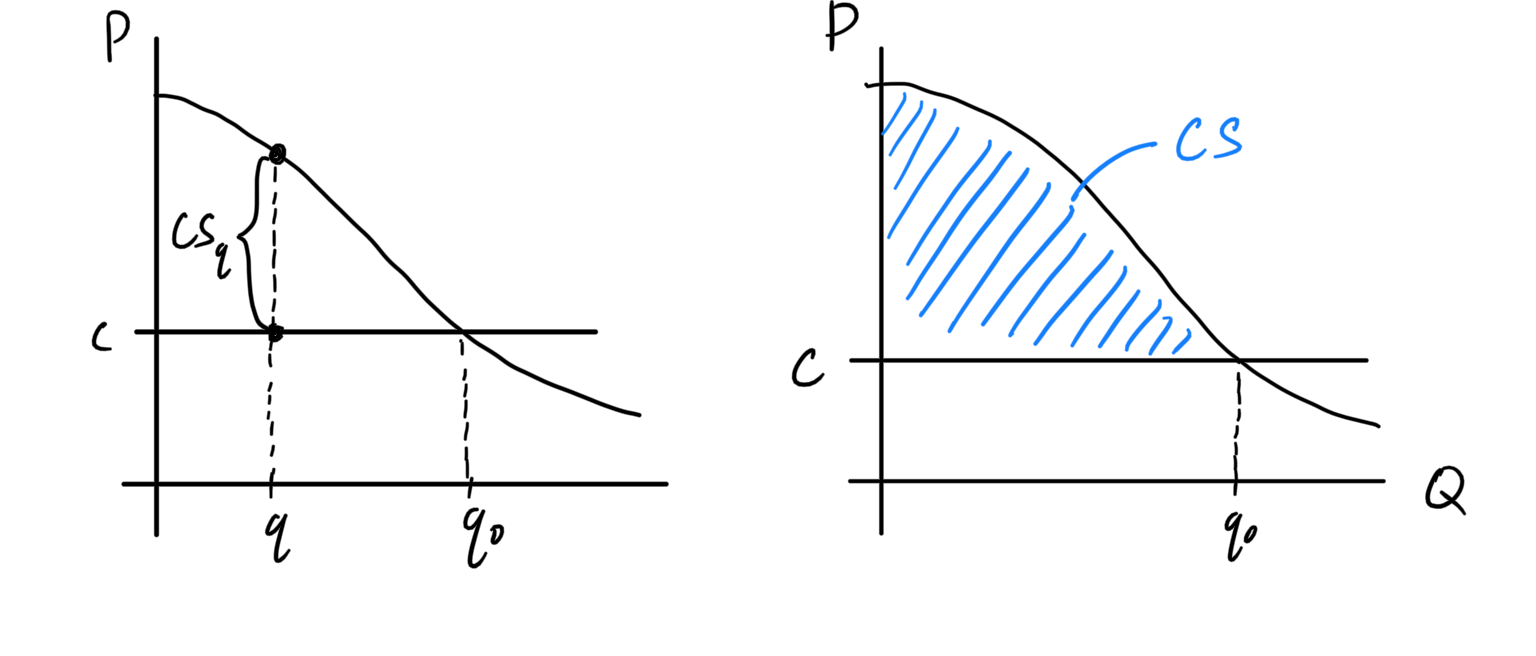
\includegraphics[scale=0.25]{img/Consumer_Surplus_Definition.PNG}
      \end{center}
    \end{definition}

    Now, we introduce a related function, the demand curve. Note that the marginal value function inputs a quantity $q$ and outputs the marginal value of $q$ (i.e. what the next unit of $\mathfrak{g}$ is worth).

    \begin{definition}[Demand Function]
      The demand function $D$ is a function
      \[D: \text{actual price } c \text{ of } \mathfrak{g} \mapsto q_0 \text{ wanted to maximize consumer surplus}=\text{quantity demanded} \]
      In other words, given the actual price $c$ for a unit of good $\mathfrak{g}$, it is clear that the consumer can buy up to $q_0$ units of $\mathfrak{g}$ in order to achieve maximum consumer surplus. The quantity of $\mathfrak{g}$ demanded by the consumer would be $q_0$. Note that
      \begin{enumerate}
        \item the consumer would not want to demand more than $q_0$ since that would lead to negative value (marginal value is less than cost) 
        \item the consumer would not want to demand less than $q_0$ since there is extra room for profit.  
      \end{enumerate}

      Note that both $D$ and $v_M$ represents the same curve in $Q \times P$, but they are inverses
      \[D = v_M^{-1}\]
      Therefore, we can just think of the demand function as taking in cost and outputting the demanded quantity. This is represented in the \textbf{demand curve}. 
      \begin{center}
        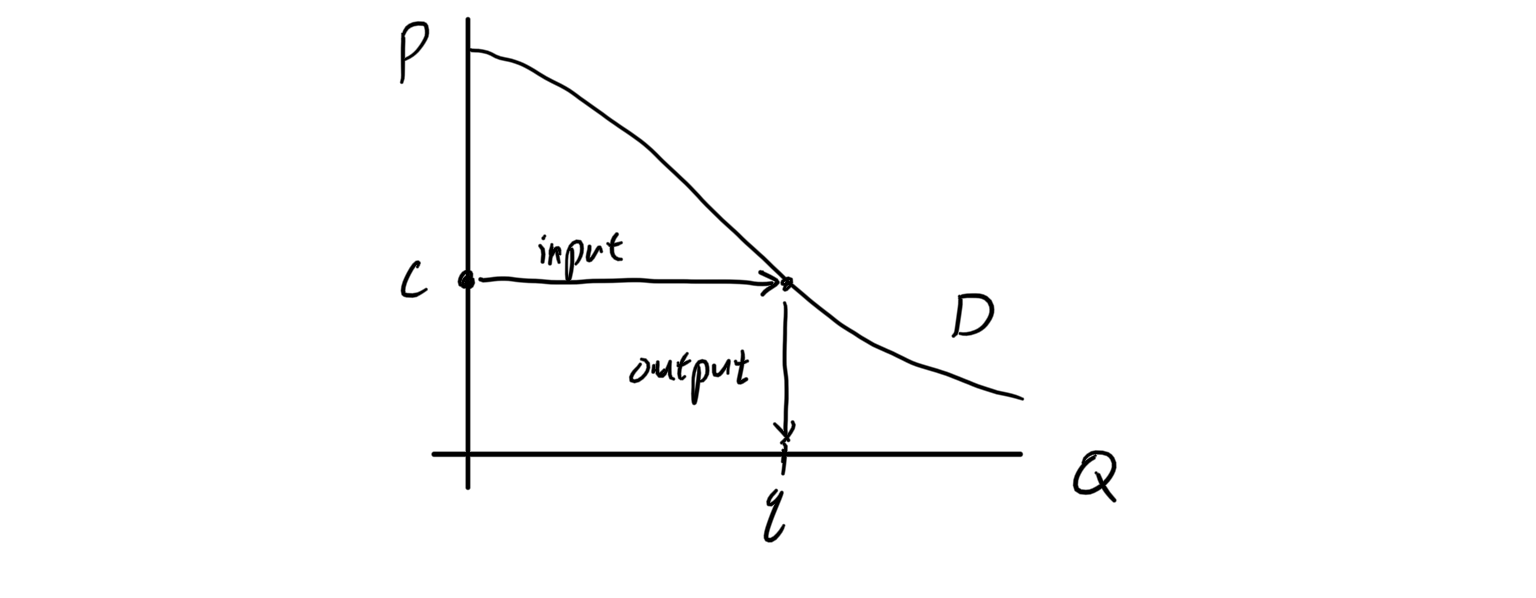
\includegraphics[scale=0.25]{img/Demand_Curve.PNG}
      \end{center}
    \end{definition}

    \begin{theorem}[Law of Demand]
      The \textbf{law of demand} states that for a consumer, the quantity $q$ demanded for a certain good is inversely proportional to the price $p$ of that good, assuming all else being equal. That is, 
      \begin{align*}
        \text{increase in price } & \implies \text{ decrease in quantity demanded} \\
        \text{decrease in price } & \implies \text{ increase in quantity demanded}
      \end{align*}
      In simple terms, we can interpret this law as such. If the price for a certain good goes down, the consumers, with the same money, have more buying power to buy more quantities. Hence, the quantity demanded increases. 
    \end{theorem}
    \begin{proof}
      This is quite easy to see with our current tools. Given a price $p_0$ and $q_0 = D (p_0)$, say the cost increases to $p_I$. Since the demand curve (interpreted as a marginal value curve) is unchanged, the marginal returns net of marginal cost decreases, lessening the consumer surplus $CS_q$ for each $q$. But if $CS_q$ is lessened for all $q$, then it would approach $0$ faster as $q$ increases, meaning that quantity demanded $q_I$ would decrease. The same logic can be applied to proving that a decreased cost leads to an increase in quantity demanded. 
      \begin{center}
        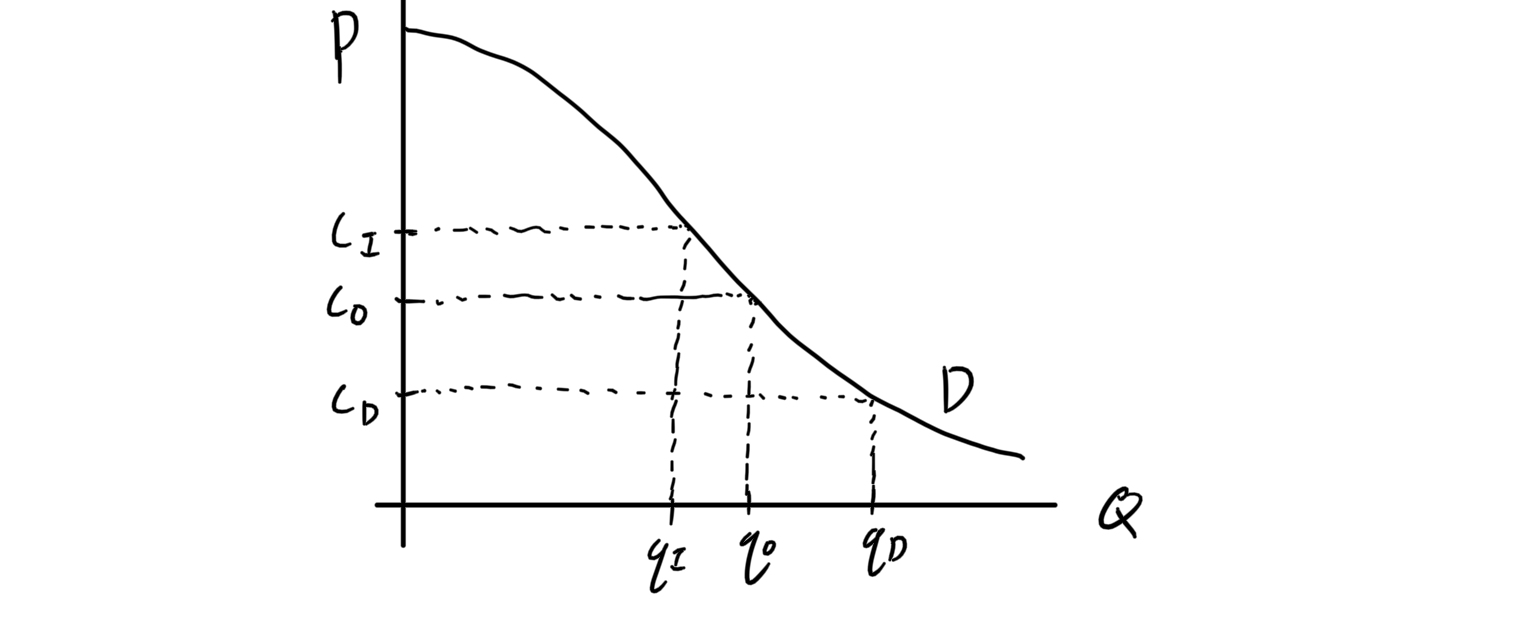
\includegraphics[scale=0.22]{img/Cost_vs_Quantity_Demand_Curve.PNG}
      \end{center}
    \end{proof}

    Note that all else being equal, if the cost changes, the quantity demanded changes inversely. However, there are external factors that can shift the entire demand curve. 

    \begin{definition}[Shift in Demand]
      External forces can change our needs for certain goods, increasing or decreasing their demand. An increase in demand is represented by an upwards/rightwards shift of the demand curve. This can be interpreted equivalently as: 
      \begin{enumerate}
        \item more units demanded at a given price, or 
        \item a higher willingness to pay for each unit (i.e. higher marginal value)
      \end{enumerate}
      A decrease in demand is represented by a downwards/leftwards shift of the demand curve. This can be interpreted equivalently as 
      \begin{enumerate}
        \item less units demanded at a given price, or 
        \item a lower willingness to pay for each unit (i.e. lower marginal value) 
      \end{enumerate}
      \begin{center}
        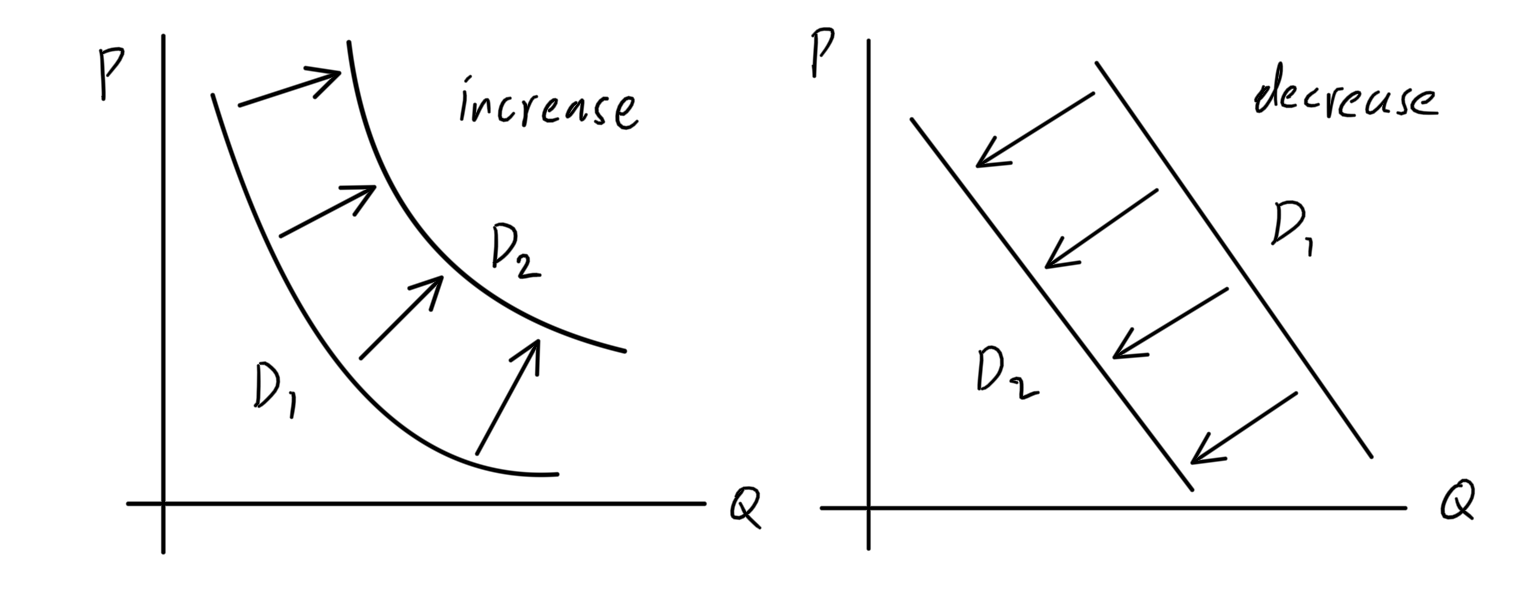
\includegraphics[scale=0.25]{img/Shift_In_Demand.PNG}
      \end{center}
    \end{definition}

    Note that there is a difference between a change is demand and a change in quantity demanded.
    \begin{enumerate}
      \item A change in demand refers to the shift in the entire demand curve
      \item A change in the quantity demanded refers to the movement of a point up and down the demand curve 
    \end{enumerate}

  \subsection{Marginal Cost Curve, Supply Curve, Producer Surplus}

    The relationship between the marginal cost and the supply is similar to that of the marginal value and the demand. The functions are inverses of each other, and represent the same graph on $P \times Q$. 

    \begin{definition}[Marginal Cost Curve]
      The \textbf{marginal cost}, denoted $c_M$, is the additional cost that it takes to produce/supply one additional unit of a good $\mathfrak{g}$. That is, 
      \[c_M: \big( \text{quantity } q \text{ of } \mathfrak{g} \big) \mapsto \big( \text{marginal cost of next unit}\]
      Marginal cost tends to increase; that is, the more units that are supplied, the more it will cost to produce an additional unit. 
      \begin{center}
          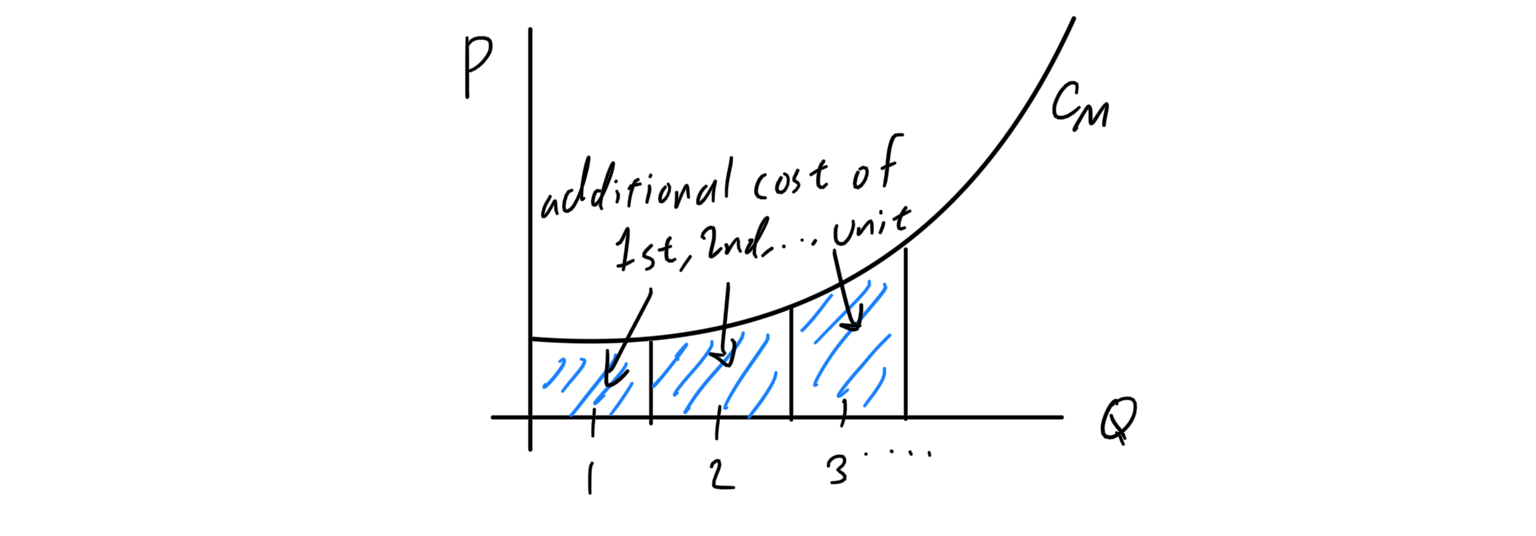
\includegraphics[scale=0.27]{img/Marginal_Cost_Curve.PNG}
      \end{center}
    \end{definition}

    Just like how consumer surplus is the marginal value net marginal (actual, constant) cost, we have an analogous definition for producer surplus. 

    \begin{definition}[Producer Surplus, Profit]
      Given the marginal cost of good $\mathfrak{g}$, a supplier would like to sell it to consumers at a constant price $c$ (analogous to how a consumer buys $\mathfrak{g}$ at price $p$). 

      The \textbf{producer surplus} is the profit/loss gotten from selling a unit of good $\mathfrak{g}$ at price $p$ net the marginal cost. As long as the price $p$ is greater than the marginal cost, then the supplier would get a net profit. Due to the monotonicity of the marginal cost function, the producer surplus is greatest on on the first supply of $\mathfrak{g}$, and then decreases to $0$ and negative values with enough supplies. Mathematically, it is defined (on the $q$th supply) 
      \[PS_q = p - c_M (q)\]
      Another definition of the producer surplus is the \textbf{maximum profit} a supplier could make. This would be found by summing up all of the individual profits until the point $q_0$, which represnts the point where the marginal profit is equal to the amrginal cost. Mathematically, it is defined
      \[PS = \int_0^{q_0} p - c_M (q) \, dq\]
      \begin{center}
        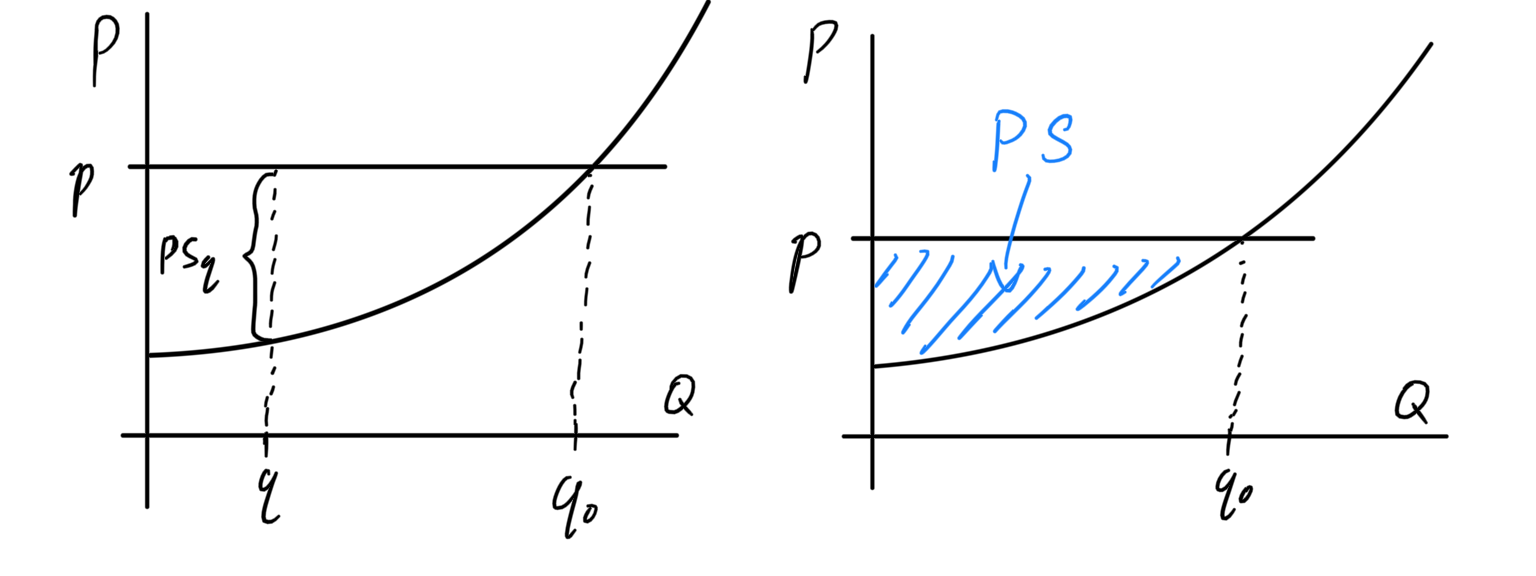
\includegraphics[scale=0.25]{img/Producer_Surplus.PNG}
      \end{center}
    \end{definition}

    \begin{definition}[Supply Function]
      The supply function $S$ is a function
      \[S: \text{actual price } c \text{ of } \mathfrak{g} \mapsto q_0 \text{ wanted to maximize producer surplus} = \text{quantity supplied}\]
      In other words, given the actual price $c$ for a unit good $\mathfrak{g}$, it is clear that the supplier can produce up to $q_0$ units of $\mathfrak{g}$ in order to achieve maximum consumer surplus. The quantity of $\mathfrak{g}$ supplied by the consumer would be $q_0$. Note that
      \begin{enumerate}
        \item the supplier would not want to supply more than $q_0$ since that would lead to a loss in money (since the marginal cost is greater than the price)
        \item the supplier would not want to supply less than $q_0$ since there is extra room for profit. 
      \end{enumerate}
      Note that both $S$ and $c_M$ represent the same curve in $Q \times P$, but they are inverses
      \[S = c_M^{-1}\]
      Therefore, we can just think of the supply function as taking in cost and outputting the demanded quantity. This is represented in the \textbf{supply curve}. 
      \begin{center}
        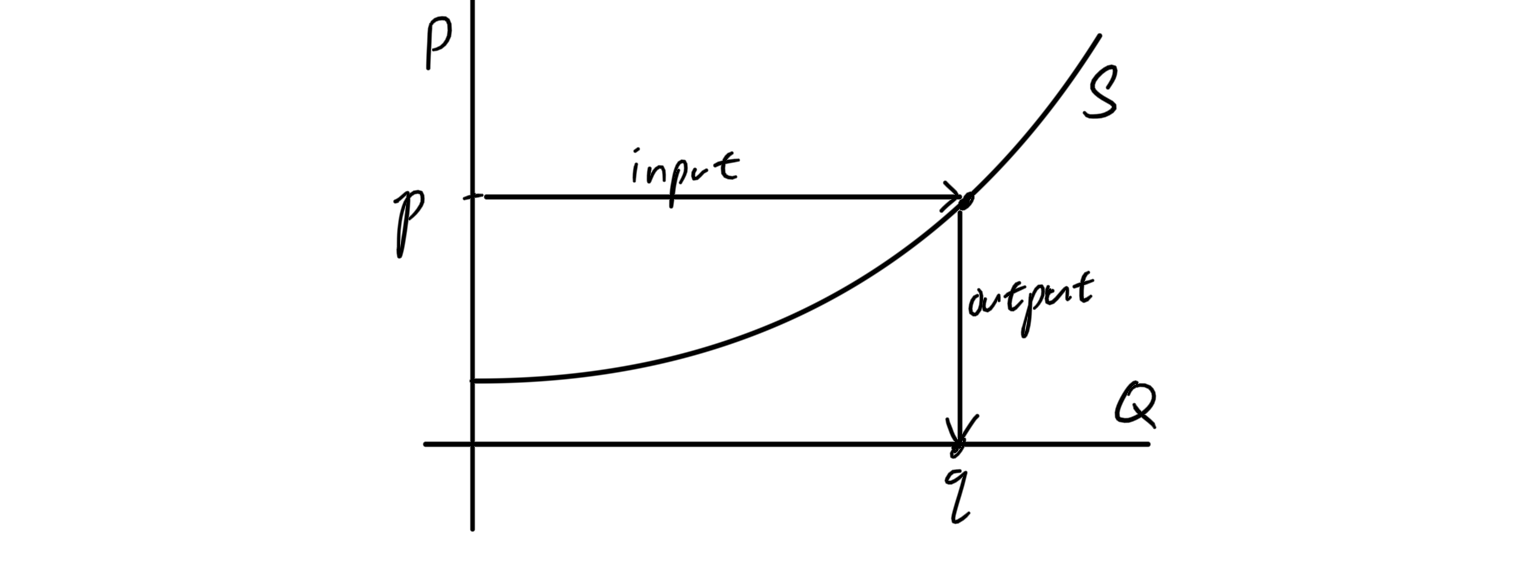
\includegraphics[scale=0.25]{img/Supply_Function.PNG}
      \end{center}
    \end{definition}

    \begin{theorem}[Law of Supply]
      The \textbf{law of supply} states that for a consumer, the quantity $q$ supplied for a certain good is proportional to the price $p$ of that good, assuming all else equal. That is, 
      \begin{align*}
        \text{increase in price } & \implies \text{ increase in quantity supplied} \\
        \text{decrease in price } & \implies \text{ decrease in quantity supplied}
      \end{align*}
      In simple terms, we can interpret the law as such: Producers are willing to offer more of a product for sale on the market at higher prices by increasing production as a way of increasing profits. 
      \begin{center}
        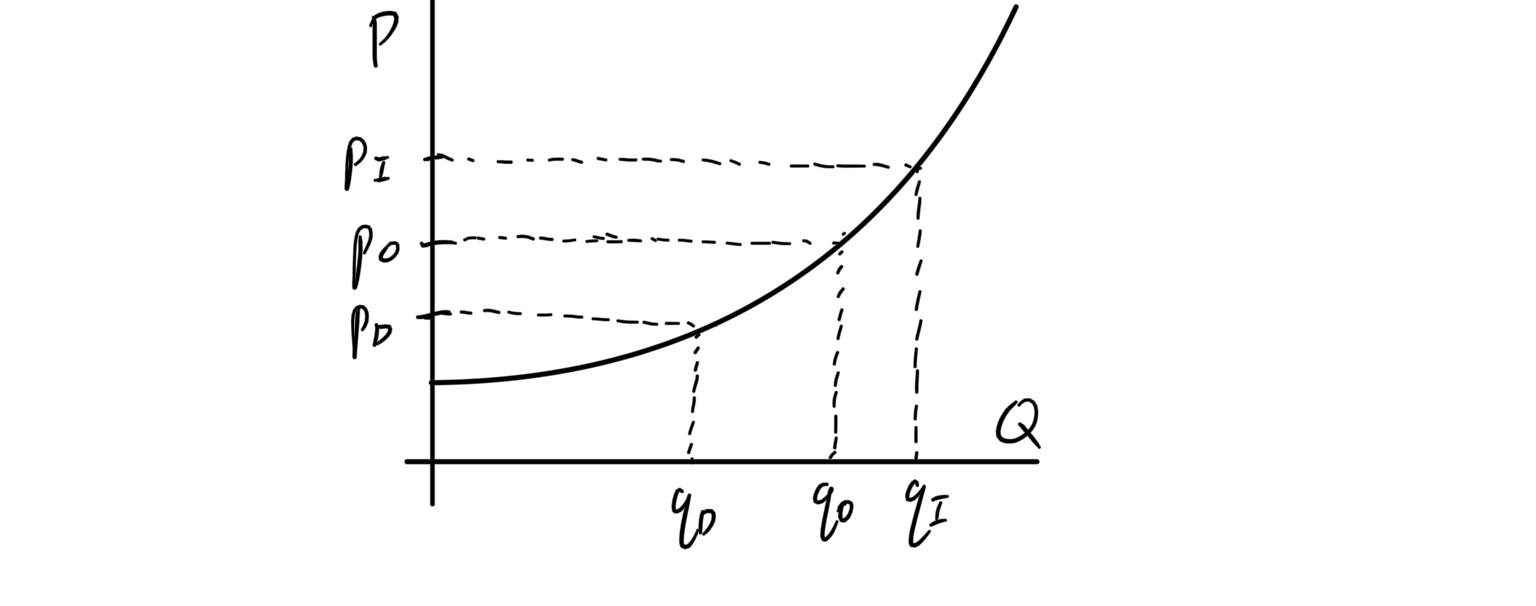
\includegraphics[scale=0.25]{img/Law_of_Supply.PNG}
      \end{center}
    \end{theorem}

    \begin{definition}[Shift in Supply]
      An increase in supply is represented by a rightwards/downwards shift of the supply curve. This can be interpreted equivalently as: 
      \begin{enumerate}
        \item more units available at a given price, or
        \item a lower price for the supply of the same number of units
      \end{enumerate}
      A decrease in supply is represented by a leftwards/upwards shift of the supply curve. This can be interpreted equivalently as: 
      \begin{enumerate}
        \item less units available at a given price, or 
        \item a higher price for the supply of the same number of units
      \end{enumerate}
      \begin{center}
        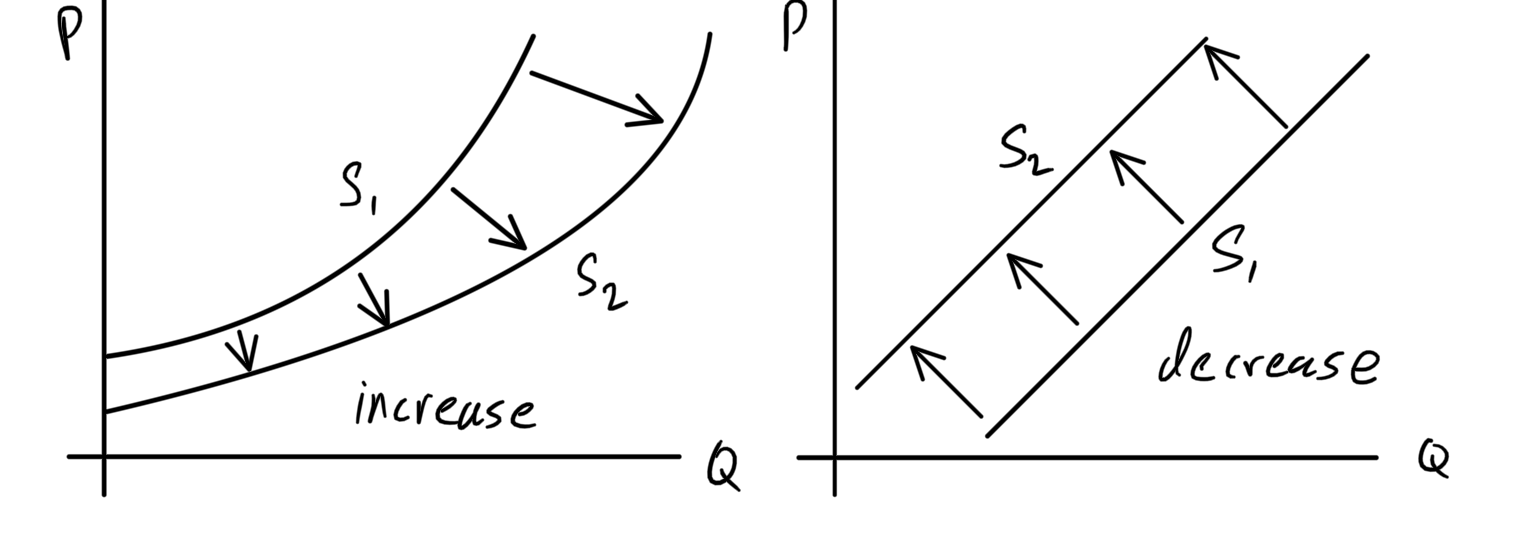
\includegraphics[scale=0.25]{img/Shift_in_Supply.PNG}
      \end{center}
    \end{definition}

  \subsection{Market Demand and Supply}

    While we have talked about individual supply and demand, we can extend this to talk about the supply and demand of the market, which refers to a population of individuals. 

    \begin{definition}[Market Demand]
      For a certain good $\mathfrak{g}$, the market demand curve of $\mathfrak{g}$ can be found by taking the \textbf{horizontal sum} of the individual market demand curves; it is a horizontal sum because we are summing up the quantities demanded at every price level. 
      \begin{center}
          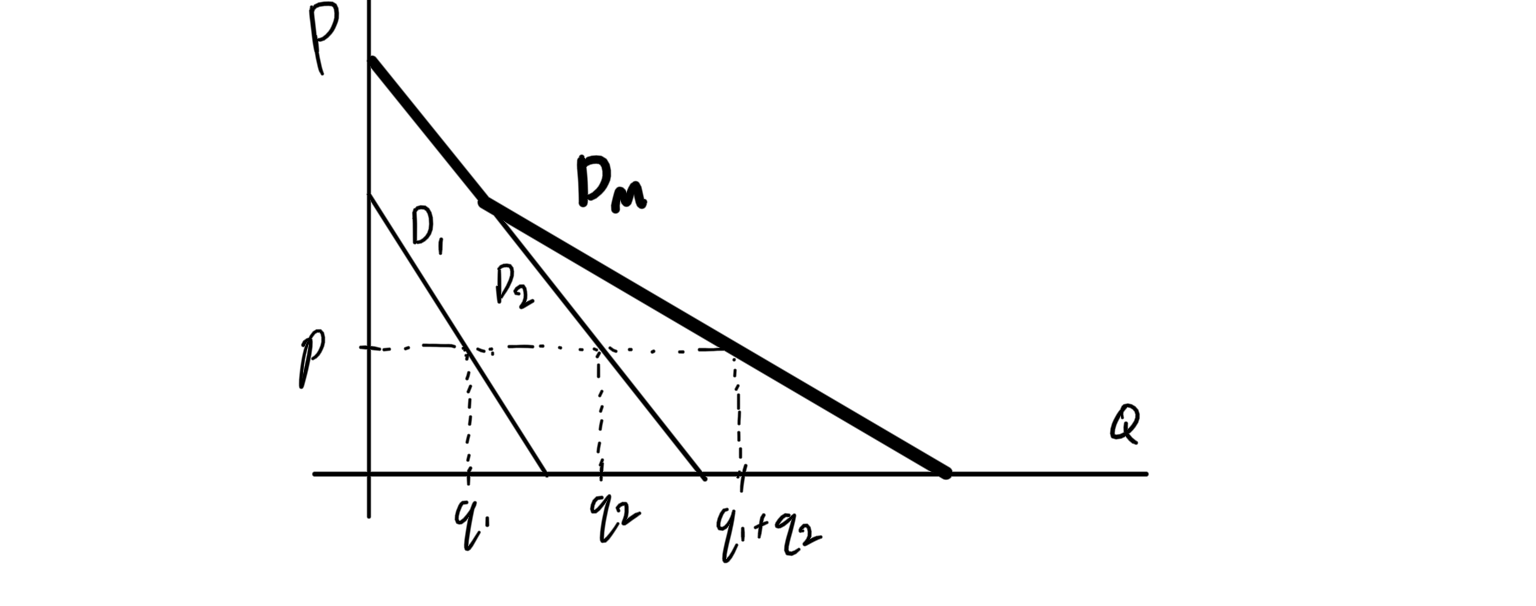
\includegraphics[scale=0.27]{img/Market_Demand.PNG}
      \end{center}
      Mathematically speaking, let there be $N$ consumers $I_1, \ldots, I_N$ in a market. At a price level of $p_0$, if consumer $I_i$ demands quantity $D_i (p_0)$ of $\mathfrak{g}$ (where $D_i$ is the demand function of the $i$th consumer), then the demand of the market $\mathcal{M}$ at the price $p_0$ is 
      \[D_\mathcal{M} (p_0) = \sum_{i=1}^N D_i (p_0)\]
    \end{definition}

    \begin{definition}[Market Supply]
      We also take the horizontal sum of the market supply curves of every supplier in the market. 
      \begin{center}
          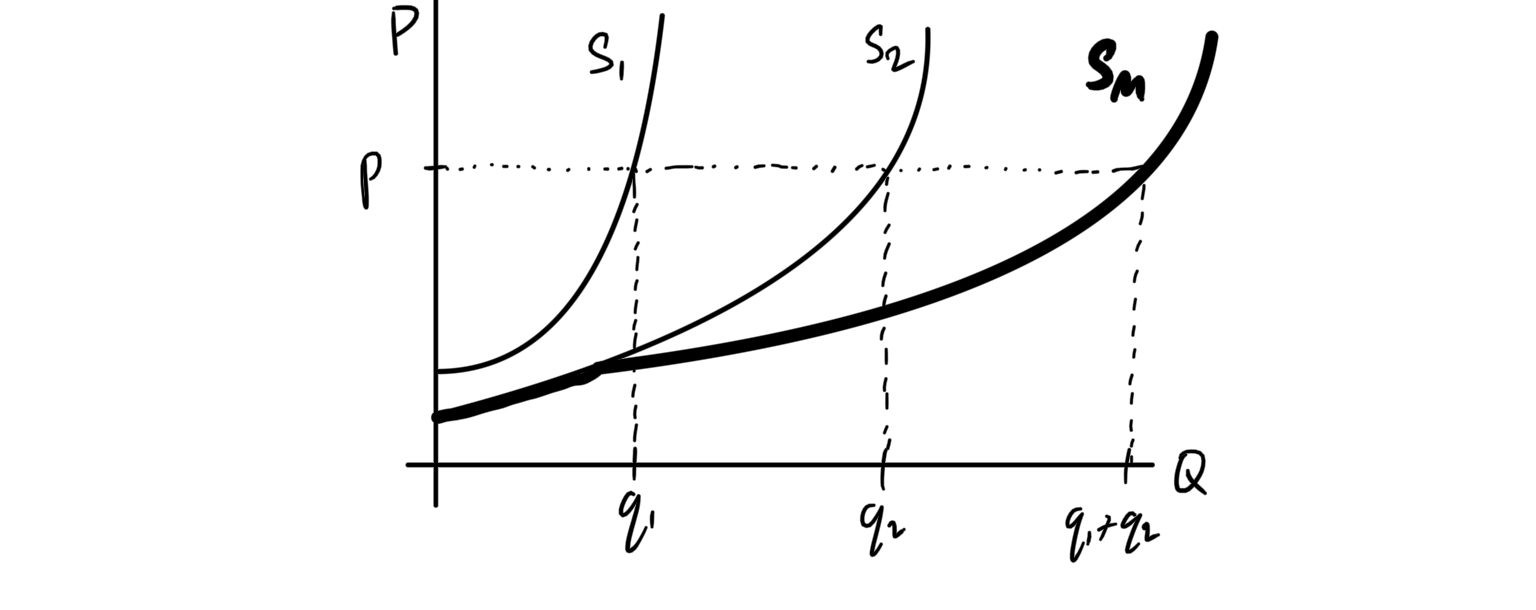
\includegraphics[scale=0.27]{img/Market_Supply.PNG}
      \end{center}
      Mathematically, let there be $M$ suppliers $I_1, \ldots, I_M$ in a market. At a price level of $p_0$, if supplier $I_i$ produces quantity $S_i (p_0)$ of $\mathfrak{g}$ (where $S_i$ is the supply function of the $i$th supplier), then the supply of the market $\mathcal{M}$ at the price $p_0$ is 
      \[S_\mathcal{M} (p_0) = \sum_{i=1}^M S_i (p_0)\]
    \end{definition}

    \subsubsection{Substitutes and Complements}

      The supplies and demands for some goods can influence those of other, related ones. 

      \begin{definition}[Normal, Inferior Goods]
        We can categorize goods as such, based on income. Usually, with an increase in income, people's demands rise for goods. 
        \begin{enumerate}
          \item Goods whose demand does not increase with income are known as \textbf{inferior goods} (e.g. bus fares). They get substituted for better quality goods. 
          \item Goods whose demand increases with income are known as \textbf{normal goods}.
        \end{enumerate}
      \end{definition}

      \begin{definition}[Complements]
        For a given good $\mathfrak{g}$, a \textbf{complementary good} $\mathfrak{h}$ is a good whose appeal increases with the popularity of its complement. We can define them more specifically within the context of demand and supply: 
        \begin{enumerate}
          \item If the price of $\mathfrak{h}$ decreases, then the quantity demanded for $\mathfrak{h}$ increases. This causes the demand of complementary good $\mathfrak{g}$ to increase. Similarly, the price of $\mathfrak{h}$ increasing causes the quantity demanded to decrease, resulting in the demand of $\mathfrak{g}$ to decrease. 
          \item If the price of $\mathfrak{h}$ increases, then the quantity supplied for $\mathfrak{h}$ increases. This causes the supply of complementary good $\mathfrak{g}$ to increase. Similarly, the price of $\mathfrak{h}$ decreases causes the quantity supplied to decrease, resulting the supply of $\mathfrak{g}$ to decrease. 
        \end{enumerate}
      \end{definition}

      \begin{definition}[Substitutes]
        For a given good $\mathfrak{g}$, a \textbf{substitute} $\mathfrak{h}$ is a good whose appeal decreases with the popularity of its substitute. We can define the more specifically within the context of demand and supply: 
        \begin{enumerate}
          \item If the price of $\mathfrak{h}$ decreases, then the quantity demanded for $\mathfrak{h}$ increases. This causes the demand of substitute $\mathfrak{g}$ to decrease. Similarly, the price of $\mathfrak{h}$ increasing causes the quantity demanded to decrease, resulting in the demand of $\mathfrak{g}$ to increase. 
          \item If the price of $\mathfrak{h}$ increases, then the quantity supplied for $\mathfrak{h}$ increases. This causes the quantity supplied of substitute $\mathfrak{g}$ to decrease. Similarly, the price of $\mathfrak{h}$ decreasing causes the quantity supplied to decrease, resulting in the quantity supplied of $\mathfrak{g}$ to increase. 
        \end{enumerate}
      \end{definition}

  \subsection{Equilibrium}

    \begin{definition}[Surplus]
      When the price is such that the quantity supplied of a good or service exceeds the quantity demanded, some sellers are unable to sell because fewer units are purchased than are offered. This condition is called a \textbf{surplus}. 

      The sellers who fail to sell have an incentive to sell at a lower price, which will put a downwards pressure on prices, leading them to fall. This price cutting reduces the surplus until the quantity supplied equals the quantity demanded. 
    \end{definition}

    \begin{definition}[Shortage]
      When the price is low enough that the quantity demanded exceeds the quantity supplied, a \textbf{shortage} exists. 

      In this case, some buyers fail to purchase, and these buyers have an incentive to accept a slightly higher price in order to be able to trade. This puts an upward pressure on prices, leading them to rise. This price rise reduces the shortage until the quantity supplied equals the quantity demanded. 
    \end{definition}

    \begin{definition}[Equilibrium]
      When the pressure for higher prices balances the pressure for lower prices, or when the quantity supplied is the same as the quantity demanded, the state is said to be in \textbf{equilibrium}. 

      Equilibrium is \textbf{efficient}; that is, it maximizes the gains from trade, assuming that the only people affected by any given transaction are the buyers and sellers. 
    \end{definition}

    \begin{center}
      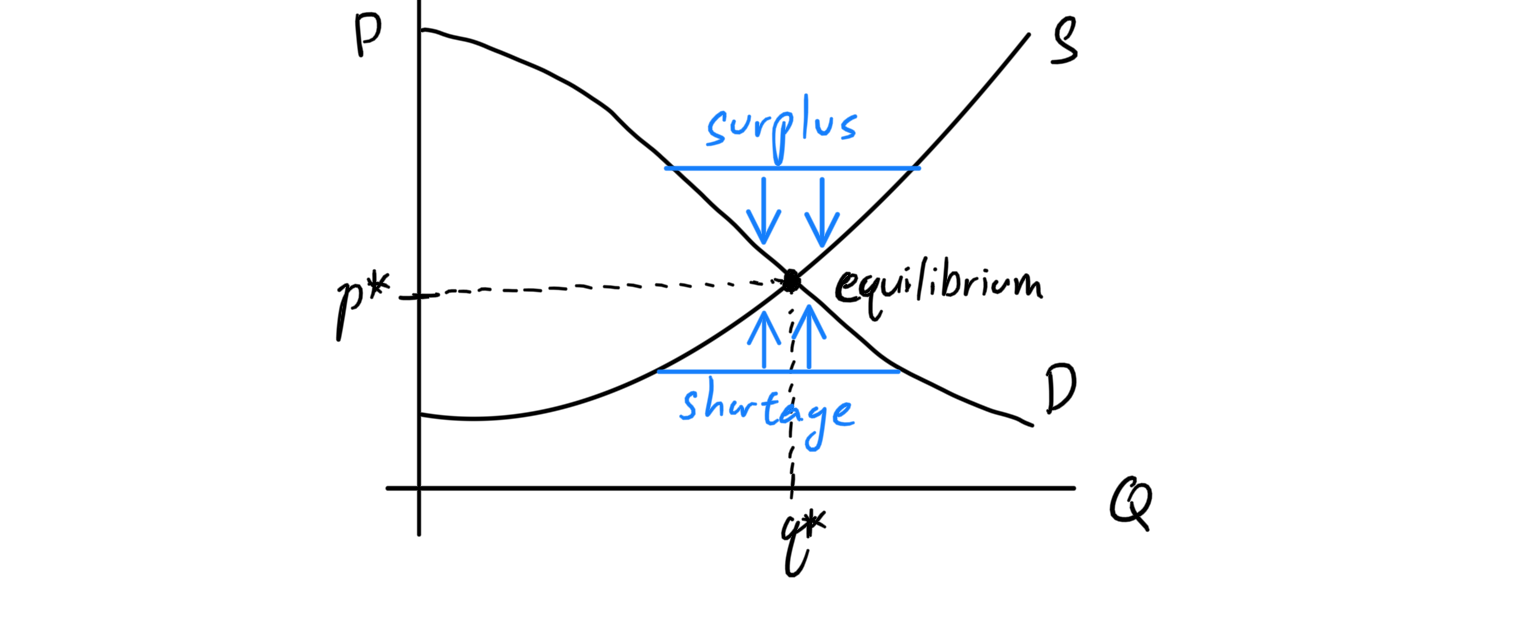
\includegraphics[scale=0.25]{img/Equilibrium_Surplus_Shortage.PNG}
    \end{center}

    \begin{definition}[Producer, Consumer Surplus at Equilibrium]
      Given that the market is at equilibrium with equilibrium price $p^*$, the consumer and producer surplus can be identified. 
      \begin{center}
        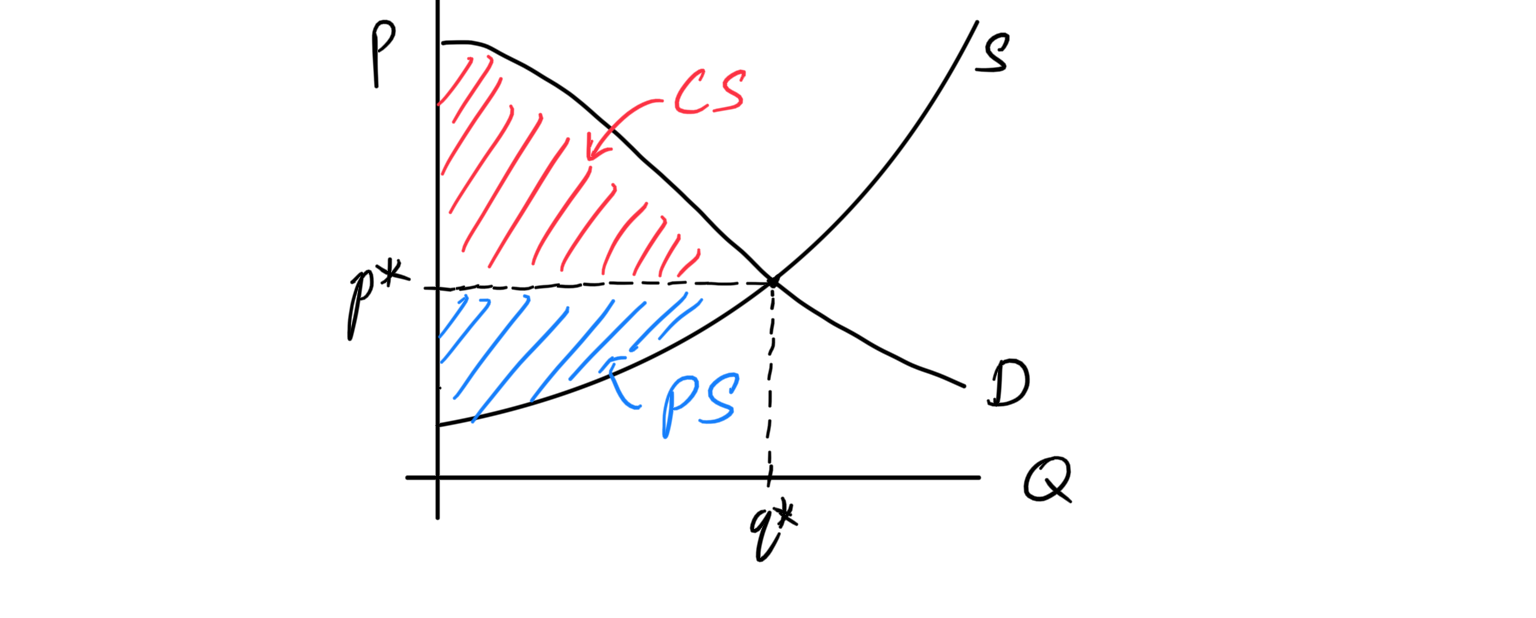
\includegraphics[scale=0.25]{img/Consumer_Producer_Surplus.PNG}
      \end{center}
      We can just think of the demand and supply curves as the marginal value and marginal cost, respectively. Given the price $p^*$ for the good, the consumers are willing to buy up to quantity $q^*$, and the suppliers are willing to supply quantity $q^*$. 
    \end{definition}

  \subsection{Changes in Supply and Demand}

    \begin{definition}[Increase in Demand]
      An increase in demand will lead to the demand curve $D_1$ shifting upwards/rightwards to a new demand curve $D_2$. 
      \begin{center}
        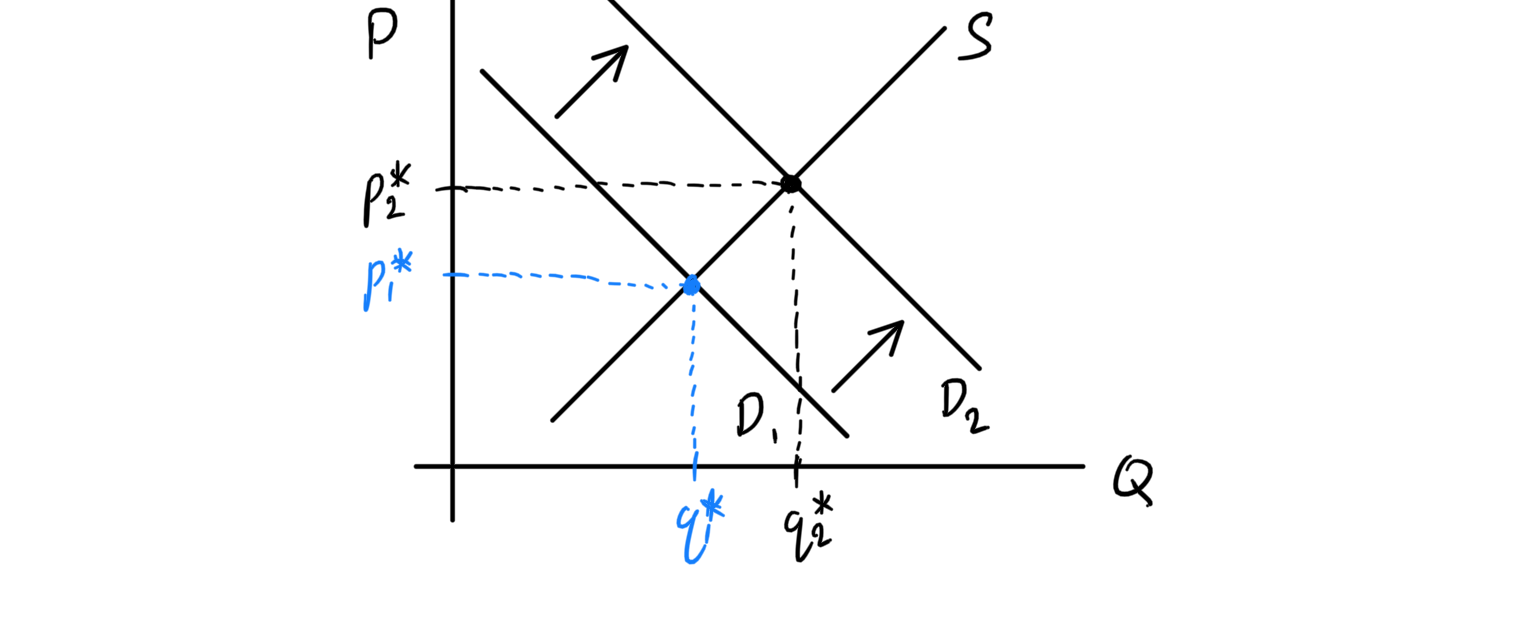
\includegraphics[scale=0.25]{img/Demand_I.PNG}
      \end{center}
      The equilibrium quantity demanded would increase from $q_1^*$ to $q_2^*$, while the equilibrium price would increase from $p_1^*$ to $p_2^*$. Indeed, this makes sense. Interpreting the demand curve as a marginal value curve, we can see that the increase in demand increases the marginal value of the good. Therefore, consumers are willing to pay \textit{more money} (increased price) for \textit{more units} of the good (increased quantity demanded). 
    \end{definition}

    \begin{example}[Stocks]
      Marathon Digital Holdings (MARA) sold for \$19.66 (closing price) on May 13, 2021. Where does this price come from? People place orders on stocks all the time, wanting to sell it at high prices and buy at low prices. When looking at the supply and demand curve of MARA stocks, we see that \$19.66 is the equilibrium price of a MARA stock. 

      Furthermore, there are thousands of people placing orders to sell MARA at prices higher than \$19.66 and to buy MARA at prices lower than \$19.66. This causes a discrepancy in these prices, and these prices aren't fulfilled until these orders meet the equilibrium. 

      External forces, such as earnings reports and news, affect the demand of MARA stocks all the time, which fluctuates the demand curve and therefore affecting the equilibrium point. A positive Q1 earnings report could increase the demand for MARA, increasing the equilibrium price (i.e. the market price) to, say \$21.11. As the demand curve goes up, all orders placed that sell MARA at prices below \$21.11 are fulfilled. 
    \end{example}

    \begin{definition}[Increase in Supply]
      An increase in supply will lead to the supply curve $S_1$ shifting downwards/rightwards to a new demand curve $S_2$. 
      \begin{center}
        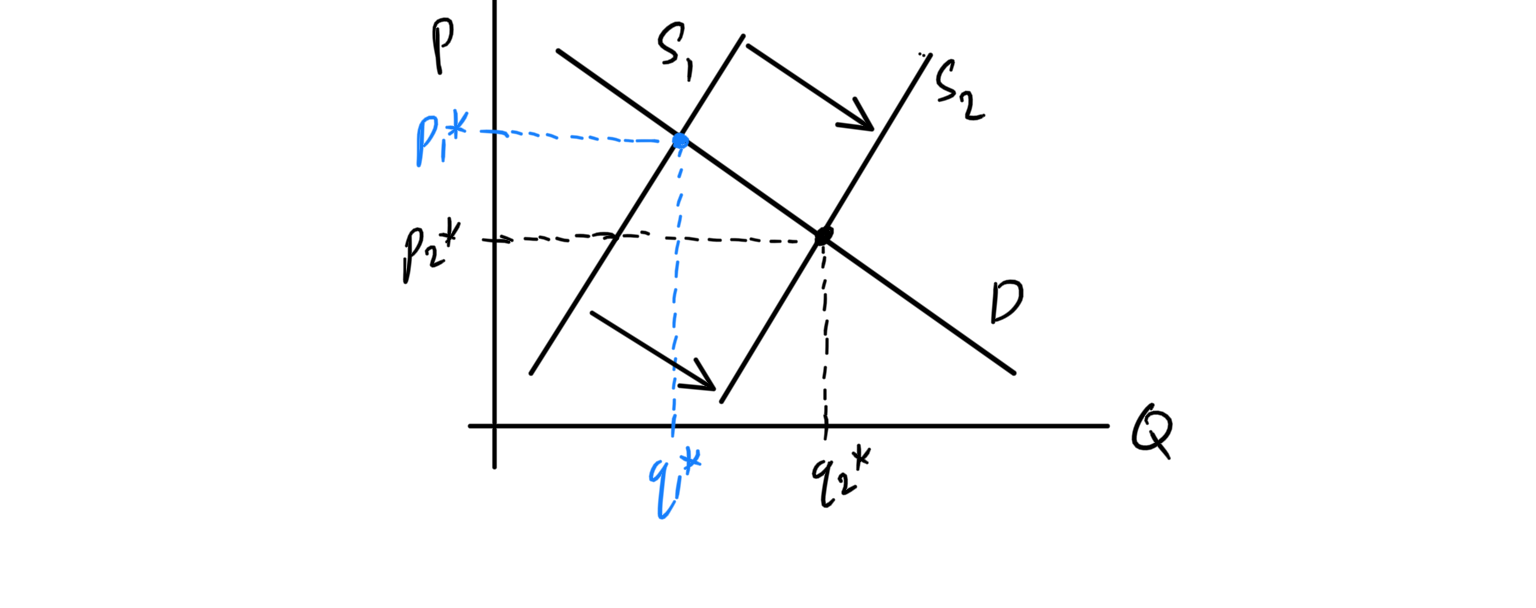
\includegraphics[scale=0.25]{img/Supply_I.PNG}
      \end{center}
      The equilibrium quantity demanded would increase from $q_1^*$ to $q_2^*$, while the equilibrium price would decrease from $p_1^*$ to $p_2^*$. Indeed, this makes sense. Interpreting the supply curve as a marginal cost curve, we can see that the increase in supply decreases the marginal cost of the good. Therefore, suppliers can produce \textit{more units} of the good (increased quantity supplied) at a \textit{lower cost} (decreased price). 
    \end{definition}

    Decreases in supply and demand can be interpreted with the same logic as above. 

    \begin{example}[Demand Increases, Supply Decreases]
      If the demand increases from $D_1$ to $D_2$ and supply decreases from $S_1$ to $S_2$ as shown below, our equilibrium point moves directly up. 
      \begin{center}
        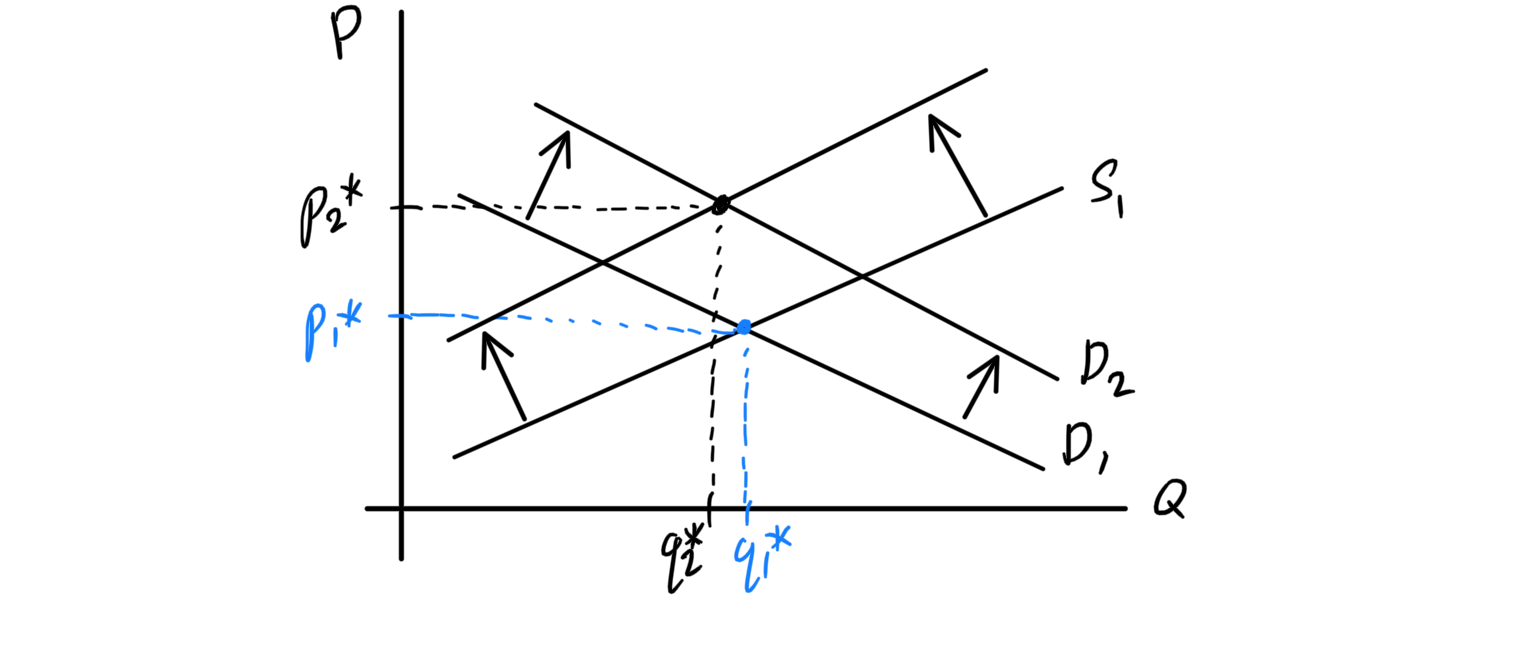
\includegraphics[scale=0.25]{img/Demand_I_Supply_D.PNG}
      \end{center}
      The increased demand increases the marginal value of the good, and the decreased supply increases the marginal cost of the good. Both of these changes drive the price up. The demand change increases the quantity demanded, while the supply change decreases the quantity supplied. 
    \end{example}

    \begin{example}[Demand Increases, Supply Increases]
      If both the demand and supply increases, the quantity demanded will doubly increase while the price will hover around the same.
      \begin{center}
        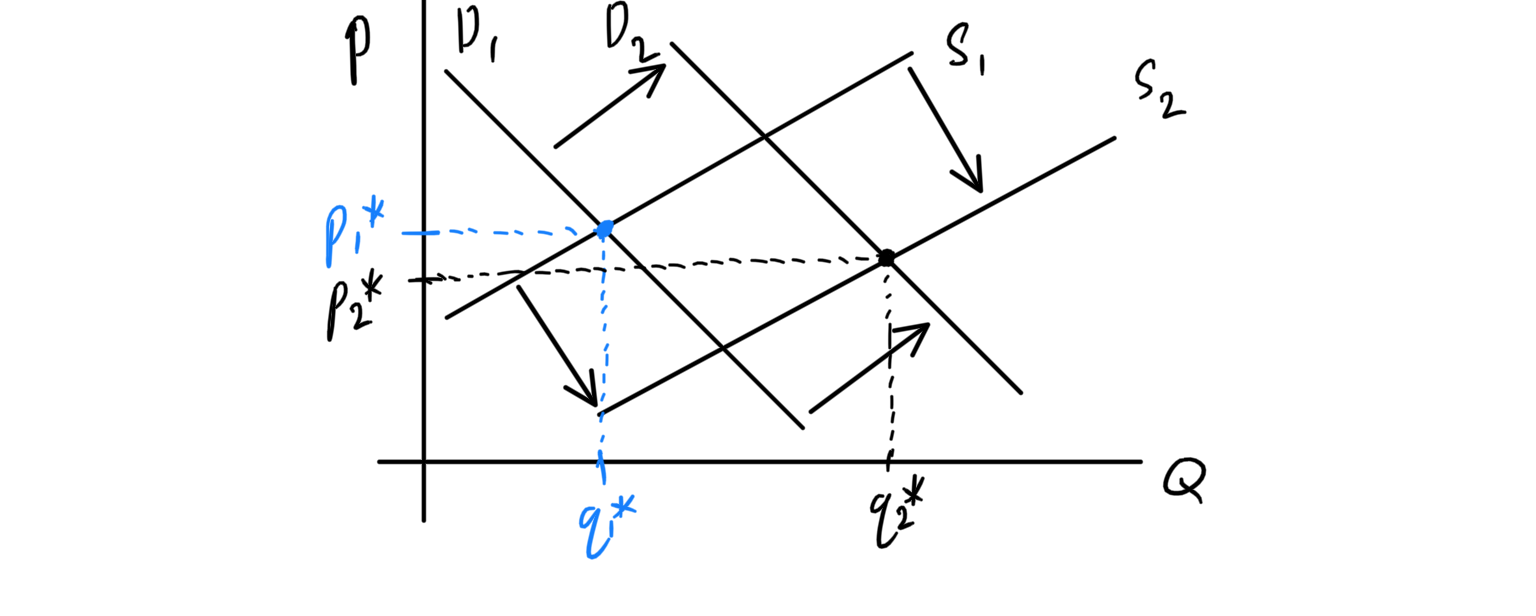
\includegraphics[scale=0.25]{img/Demand_I_Supply_I.PNG}
      \end{center}
      The increased demand and supply increases the marginal value while decreasing the marginal cost. Both contribute to the increase in quantity demanded/supplied. The demand change increases the price, while the supply change decreases the price. 
    \end{example}

  \subsection{Price Controls, Quotas}

    If the equilibrium price for a certain good or service is not sustainable, the government could intervene by setting a price control.

    \begin{definition}[Price Ceilings]
      If the price is too high (e.g. rent), then the government could set a \textbf{price ceiling} that limits how high a certain price can be for that good. 
      \begin{center}
        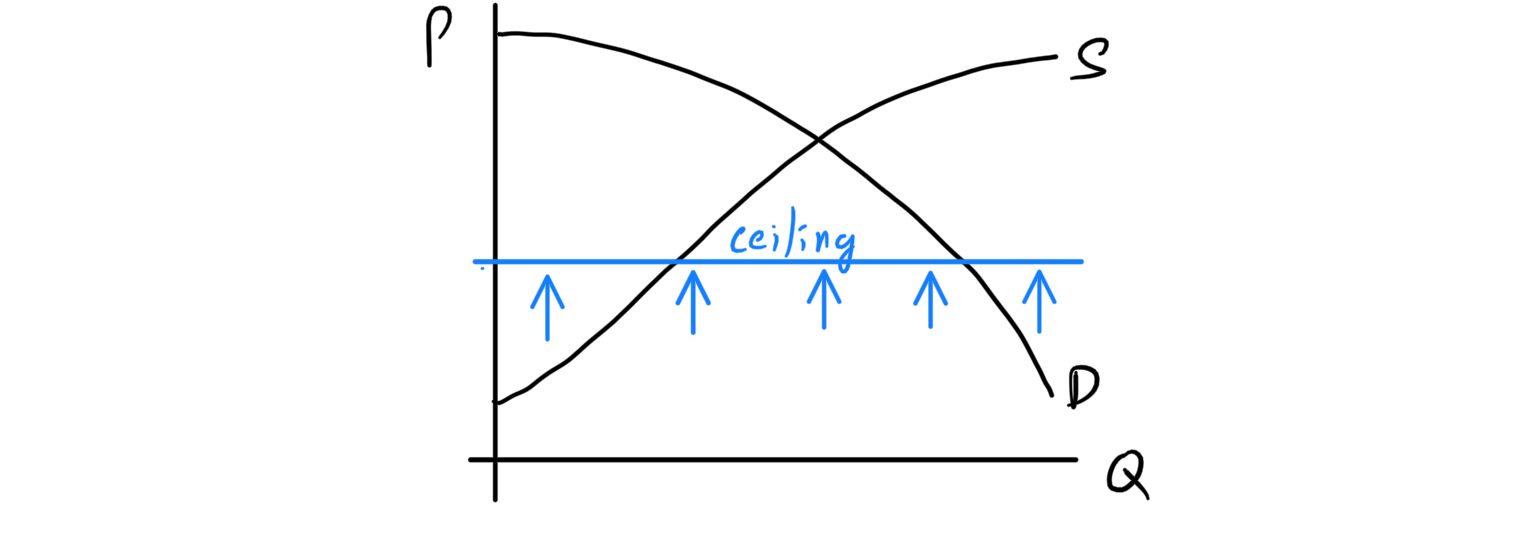
\includegraphics[scale=0.25]{img/Price_Celing.PNG}
      \end{center}
      Note that a price ceiling could cause shortages, inefficiency, and black markets. More specifically, since the actual price $p$ of the good is lower than the equilibrium price $p^*$, the quantity demanded increases to $q_D$ while the quantity supplied decreases to $q_S$. Therefore, since suppliers are only willing to sell $q_S$ units of good (due to price), this leaves extra demand (a shortage). That is, the consumer and producer surplus can only extend up to quantity $q_S$ (and not up to $q^*$). This can hurt both parties since they are restricted from maximizing their surplus/profit, and the wasted opportunity cost is called the \textbf{deadweight loss}. 
      \begin{center}
        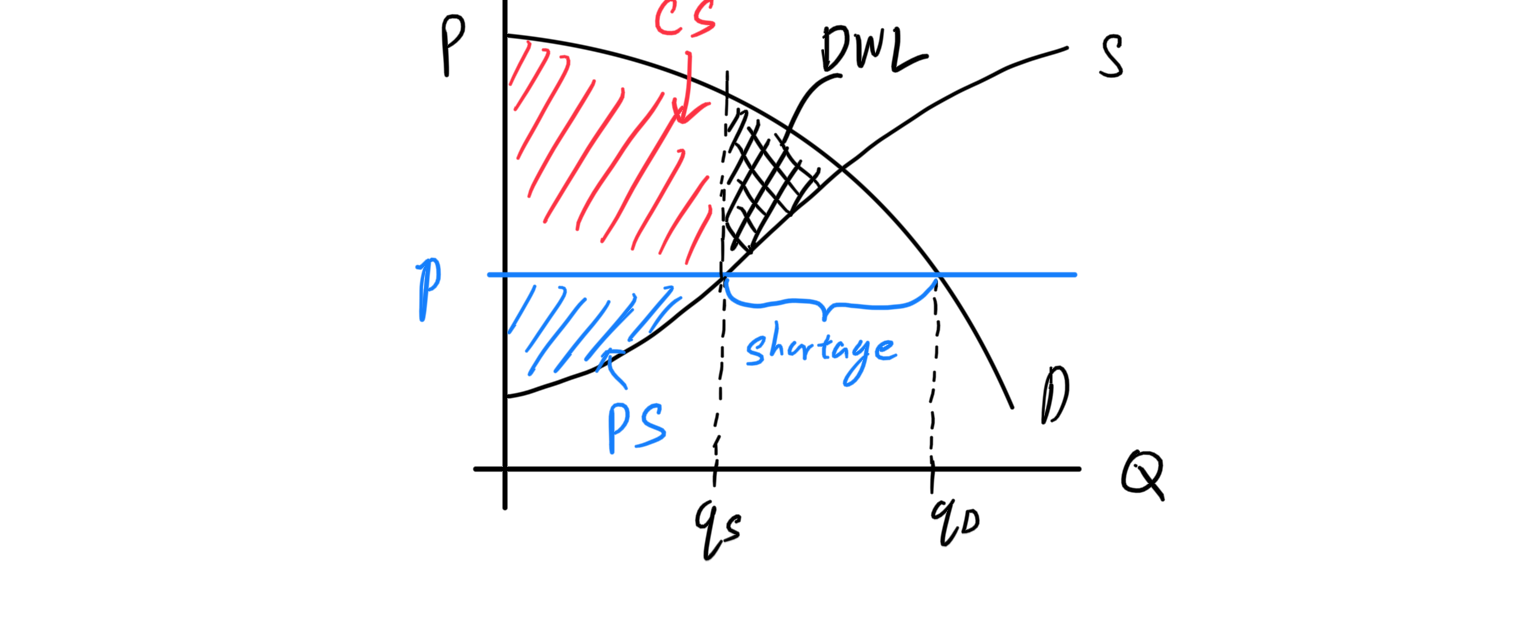
\includegraphics[scale=0.25]{img/Price_Celing_DWL.PNG}
      \end{center}
    \end{definition}

    \begin{definition}[Price Floors]
      If the price is too low (e.g. minimum wage), then the government could set a \textbf{price floor} that limits how low a certain price can be for that good. 
      \begin{center}
        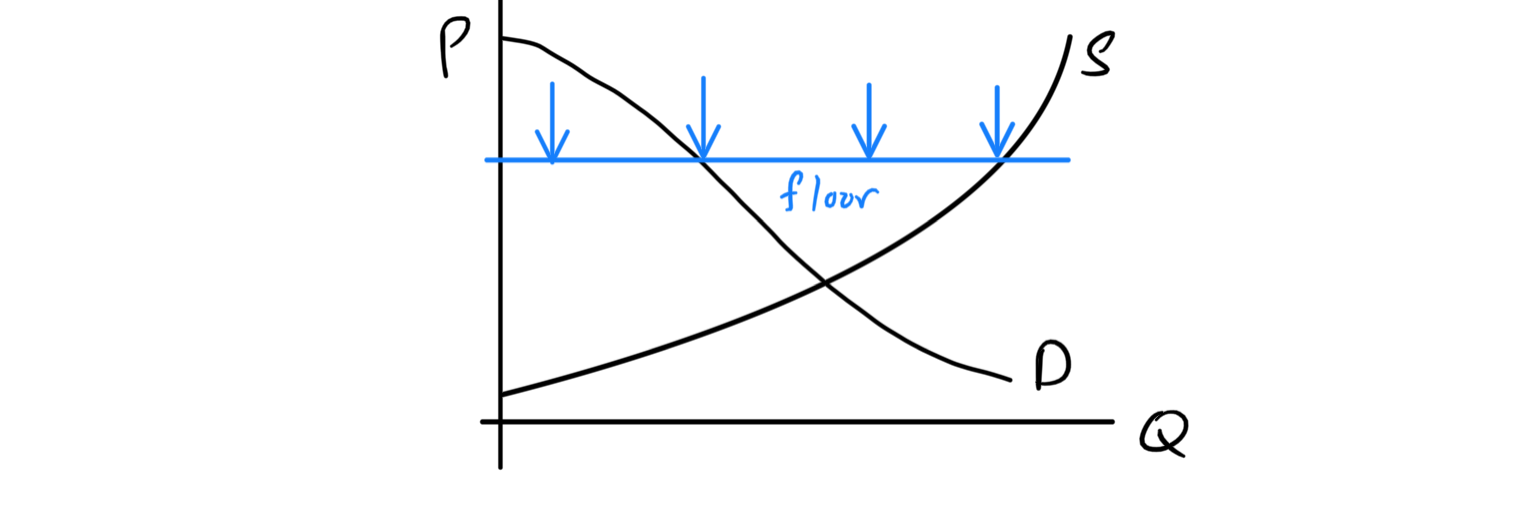
\includegraphics[scale=0.25]{img/Price_Floor.PNG}
      \end{center}
      Note that a price floor could cause surpluses, inefficiency, and wasted resources. More specifically, since the actual price $p$ of the good is higher than the equilibrium price $p^*$, the quantity demanded decreases to $q_D$ while the quantity supplied increases to $q_S$. Therefore, since consumers are only demanding up $q_D$ units of good (due to price), this leaves extra supply (a surplus). That is, the consumer and producer surplus can only extend up to quantity $q_D$ (and not up to $q^*$). This can hurt both parties since they are restricted from maximizing their surplus/profit, leading to \textbf{deadweight loss}. 
      \begin{center}
        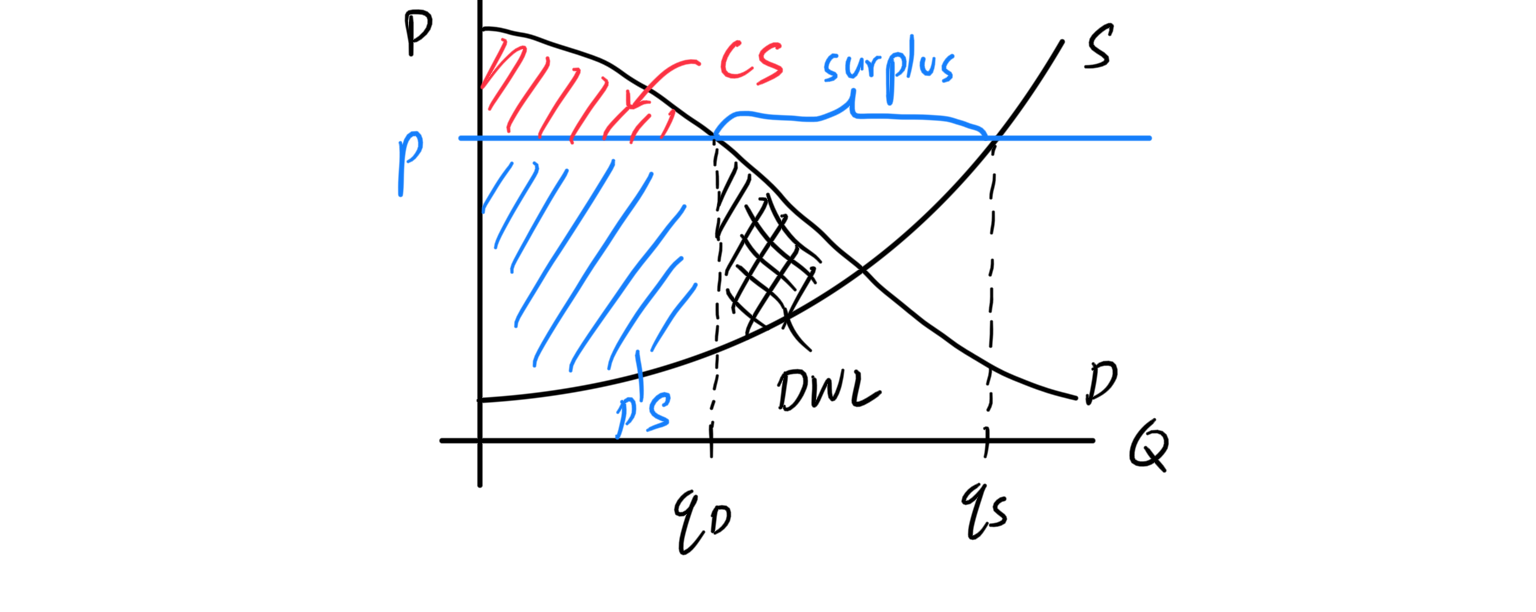
\includegraphics[scale=0.25]{img/Price_Floor_DWL.PNG}
      \end{center}
    \end{definition}

    \begin{definition}[Quotas]
      A \textbf{quota}, or \textbf{quantity control}, is an upper limit on the quantity of some good that can be bought or sold. 
      \begin{center}
        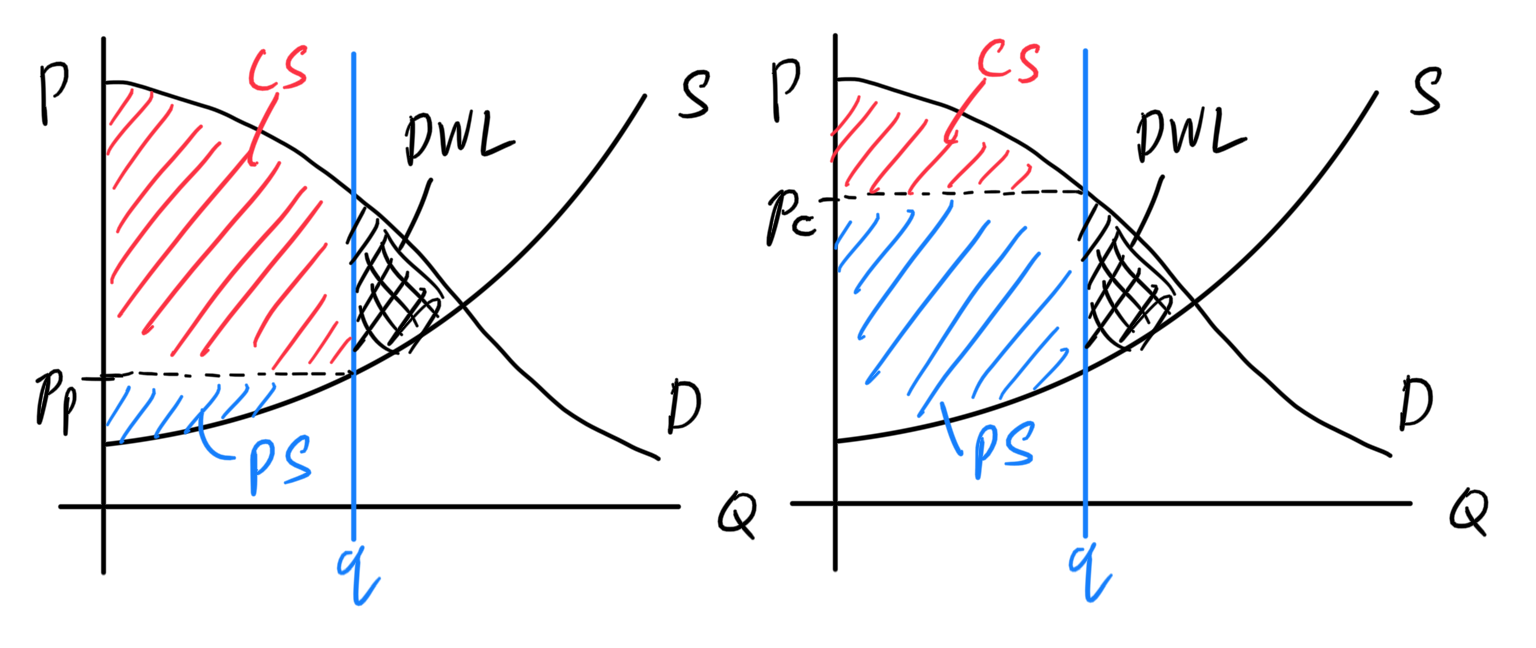
\includegraphics[scale=0.25]{img/Quota_DWL.PNG}
      \end{center}
      Since the quantity is limited, we have a bit of an instability. As long as the price is at or below $p_C$ consumers are willing to demand $q$ quantity of the good, and as long as the price is at or above $p_P$, the producers are willing to supply $q$ quantity of the good. Because of this quota, there is both a downward and upward pressure on the price of the good, but it will always remain in between $p_P$ and $p_C$. However, the deadweight loss of not being able to increases consumer/producer surplus from the quota is still there. 
    \end{definition}

  \subsection{Elasticities}

    In general, elasticity refers to the rate at which a value is affected by a change in another value. Technically, the \textbf{x-elasticity of y} measures the fractional response of $y$ to a fractional change in $x$. 

    \begin{definition}[Price-Elasticity of Demand]
      For a certain good $\mathfrak{g}$, its \textbf{elasticity} refers to how sensitive the quantity demanded is to a change in its price. That is, 
      \begin{enumerate}
        \item If a price change of $\mathfrak{g}$ leads to a greater change in quantity demanded, then $\mathfrak{g}$ is said to be \textbf{elastic}. 
        \item If a price change of $\mathfrak{g}$ leads to a smaller change in quantity demanded, then $\mathfrak{g}$ is said to be \textbf{inelastic}. 
      \end{enumerate}
      It makes sense, then, to define the price elasticity of demand as 
      \[\frac{\partial q}{\partial p} = \frac{\partial (\text{quantity demanded})}{\partial (\text{price})}\]
      However, this is sensitive to unit changes in the price or quantity, so to represent this in a unit-free formula
      \[\varepsilon = \frac{\text{\% change in quantity } q}{\text{\% change in price } p},\]
      we measure the \textit{fractional} response of $q$ to the \textit{fractional} response of $p$. That is, 
      \[\varepsilon = - \frac{d q / q}{d p / p} = - \frac{p}{D(q)} \frac{d D(p)}{dp} = - \frac{p \, D^\prime (p)}{D(p)}\]
      The negative sign is to account for the negative monotonicity of the demand curve (to make $\varepsilon$ positive). If
      \begin{enumerate}
        \item $|\epsilon| > 1$, then it is elastic and $q$ changes more than $p$. 
        \item $|\epsilon| = 1$, then it is unit elastic and $q$ changes like $p$. 
        \item $|\epsilon| < 1$, then it is inelastic and $q$ changes less than $p$. 
      \end{enumerate}
      \begin{center}
        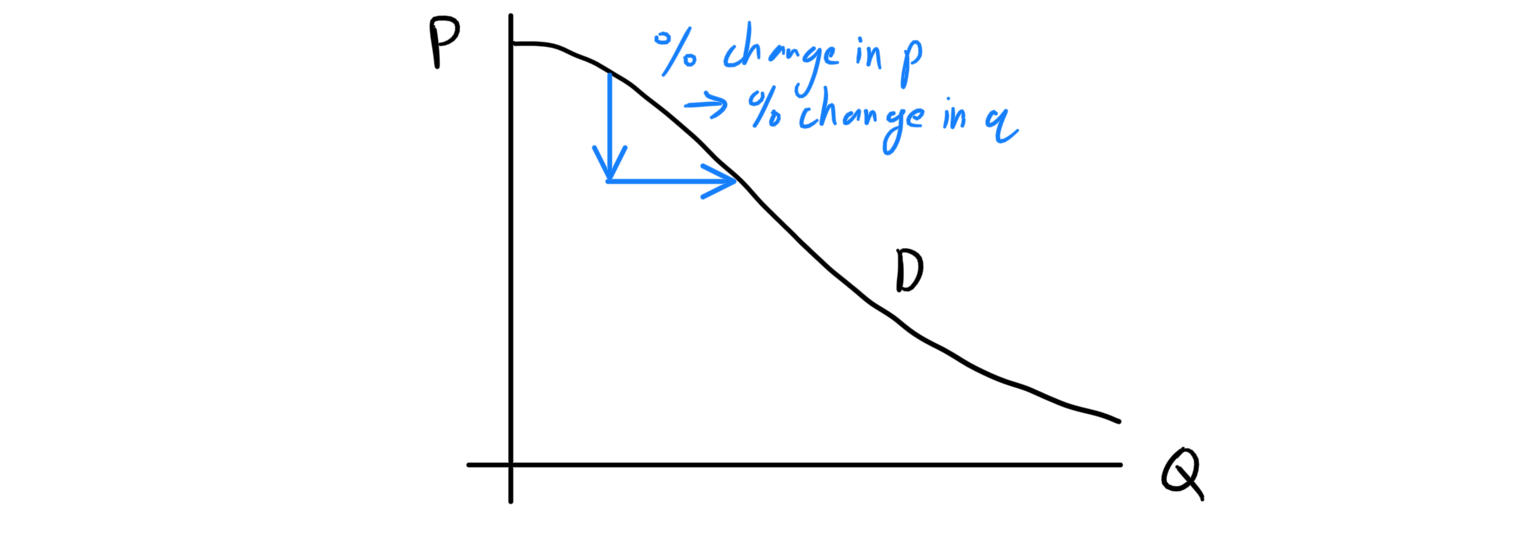
\includegraphics[scale=0.25]{img/Elasticity_Definition.PNG}
      \end{center}
    \end{definition}

    \begin{example}
      For example, suppose prices of a certain good rise by 1\%. 
      \begin{enumerate}
        \item If $\varepsilon = 0.5$, then the quantity demanded will fall by 0.5\%.
        \item If $\varepsilon = 1$, then the quantity demanded will fall by 1\%.
        \item If $\varepsilon = 2$, then the quantity demanded will fall by 2\%.
      \end{enumerate}
    \end{example}

    \subsubsection{Demand Curves with Various Elasticities}

      \begin{definition}[Linear Demand Curve]
        Counterintuitively, a linear demand curve has a varying elasticity. When the price is high (and quantity demanded low), the elasticity is high; that is, a small decrease in price from the current price would add a significant portion of the current quantity demanded. Right at the midpoint, we would have unit elasticity. As the point moves further down, it would become more and more inelastic since a small decrease in price from the current price would add an even less significant portion of the current current quantity demanded. 
        \begin{center}
          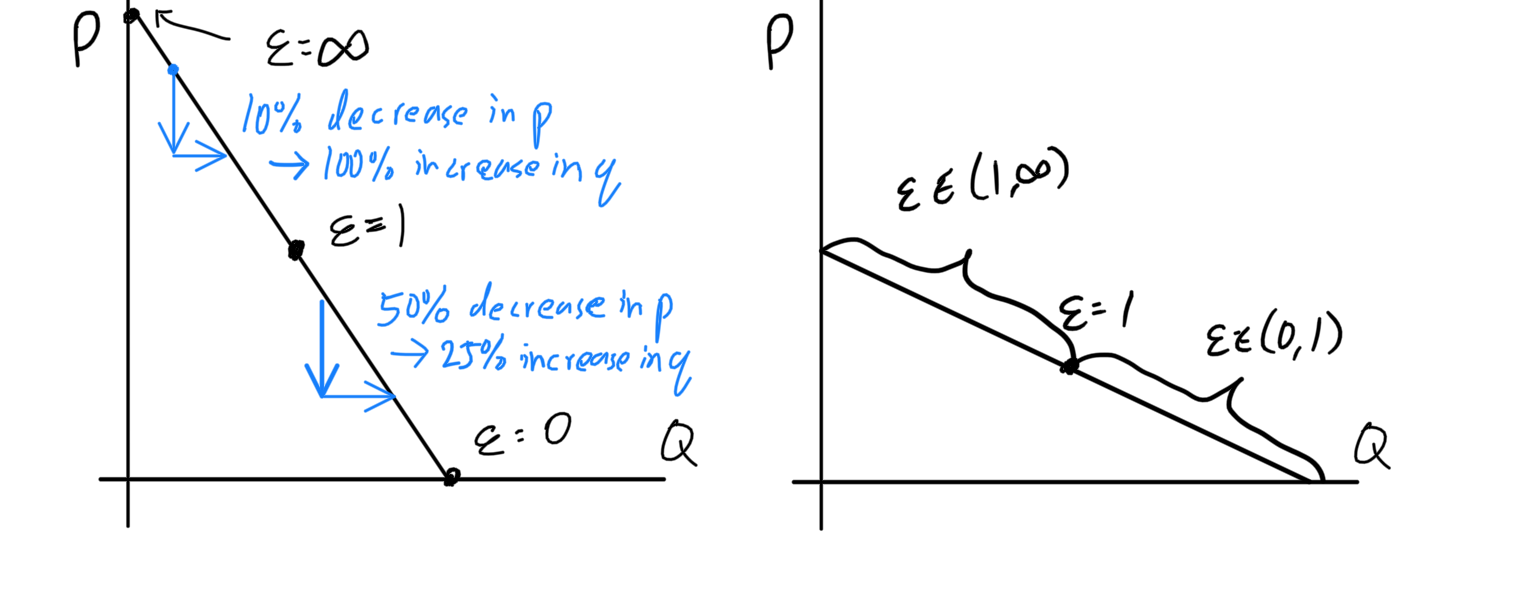
\includegraphics[scale=0.25]{img/LInear_Curve_Elasticity.PNG}
        \end{center}
      \end{definition}

      \begin{definition}[Constant Elasticity Demand Curve]
        A demand curve with constant elasticity looks like a rational function. 
        \begin{center}
          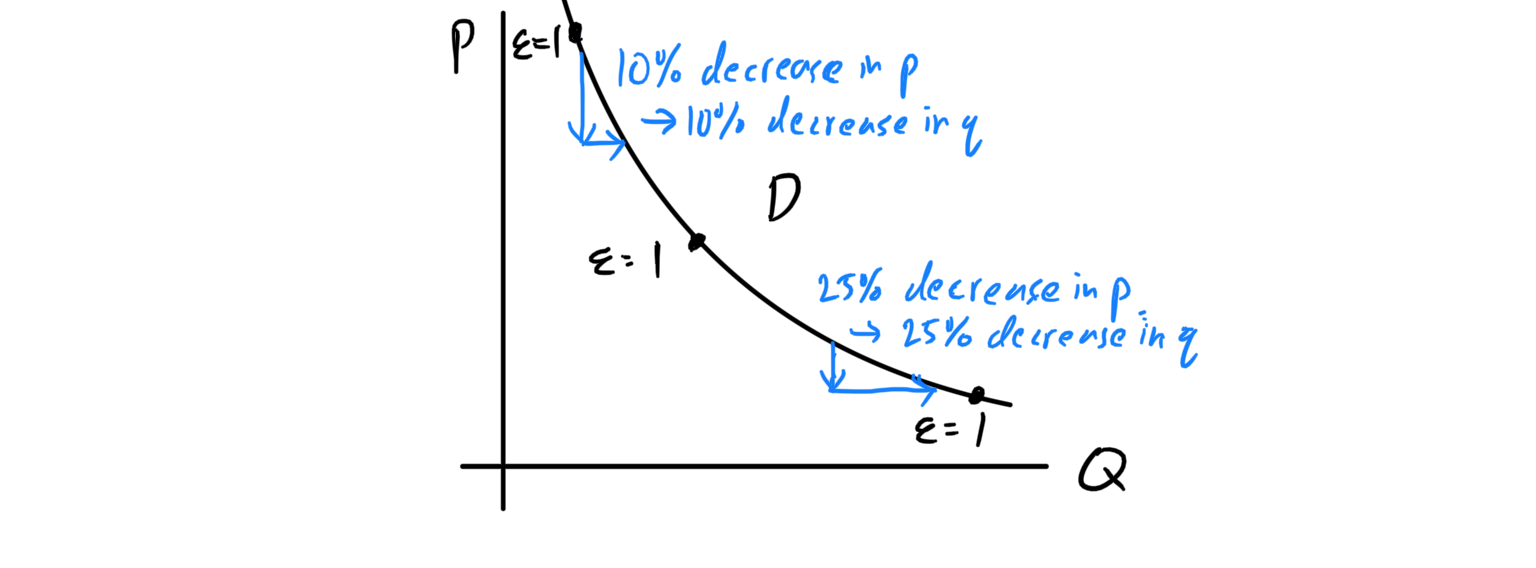
\includegraphics[scale=0.25]{img/Constant_Elasticity.PNG}
        \end{center}
      \end{definition}

      \begin{definition}[Perfectly Elastic Demand Curve]
        If the elasticity $\varepsilon = \infty$, then the quantity demanded has an infinite response to price change. This is called \textbf{perfect elasticity}. A small increase in the price of a good will cause the quantity demanded to drop to $0$. 
        \begin{center}
          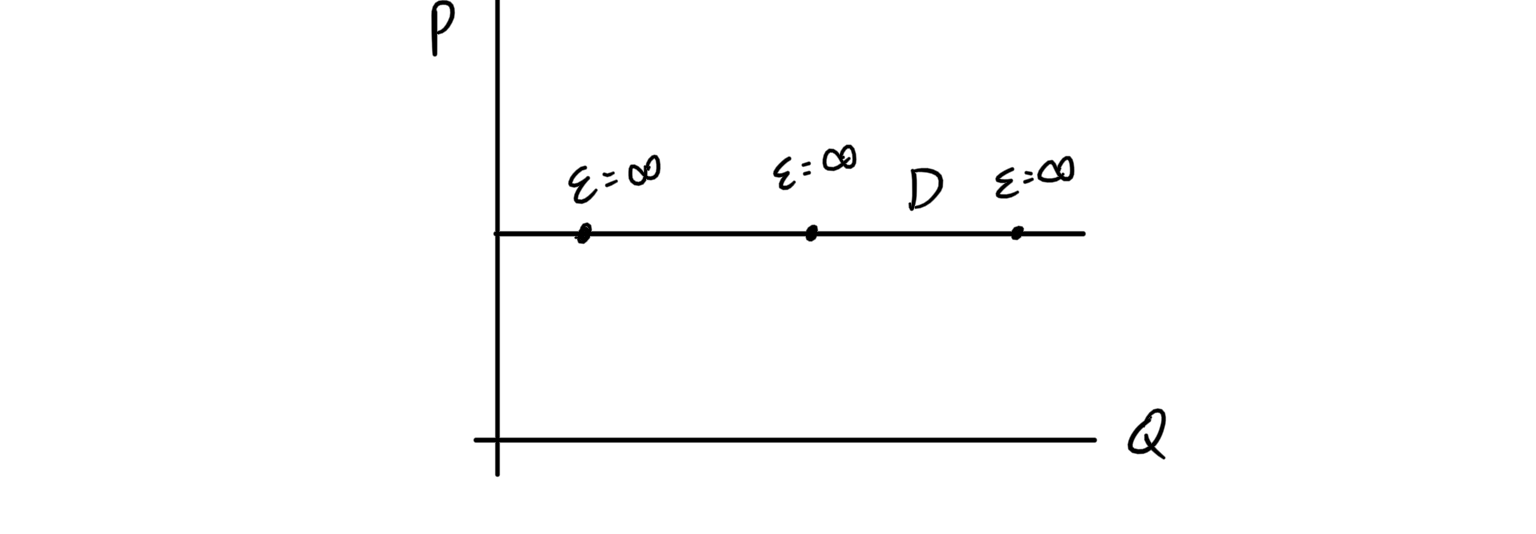
\includegraphics[scale=0.25]{img/Perfectly_Elastic.PNG}
        \end{center}
        An apple company can try to increase the price of apples from \$0.50/kg to \$0.55/kg. Since there are other companies selling apples for a cheaper price, consumers will not purchase apples from this company, dropping the quantity demanded to $0$. Note that in this scenario, we are talking about the demand curve representing the apple company and its customers, not the entire apple market. 
      \end{definition}

      \begin{definition}[Perfectly Inelastic Demand Curve]
        If the elasticity $\varepsilon = 0$, then the quantity demanded has no response to a price change. This is called \textbf{perfect inelasticity}. Even a large increase in the price of a good will not cause the quantity demanded to change at all. 
        \begin{center}
          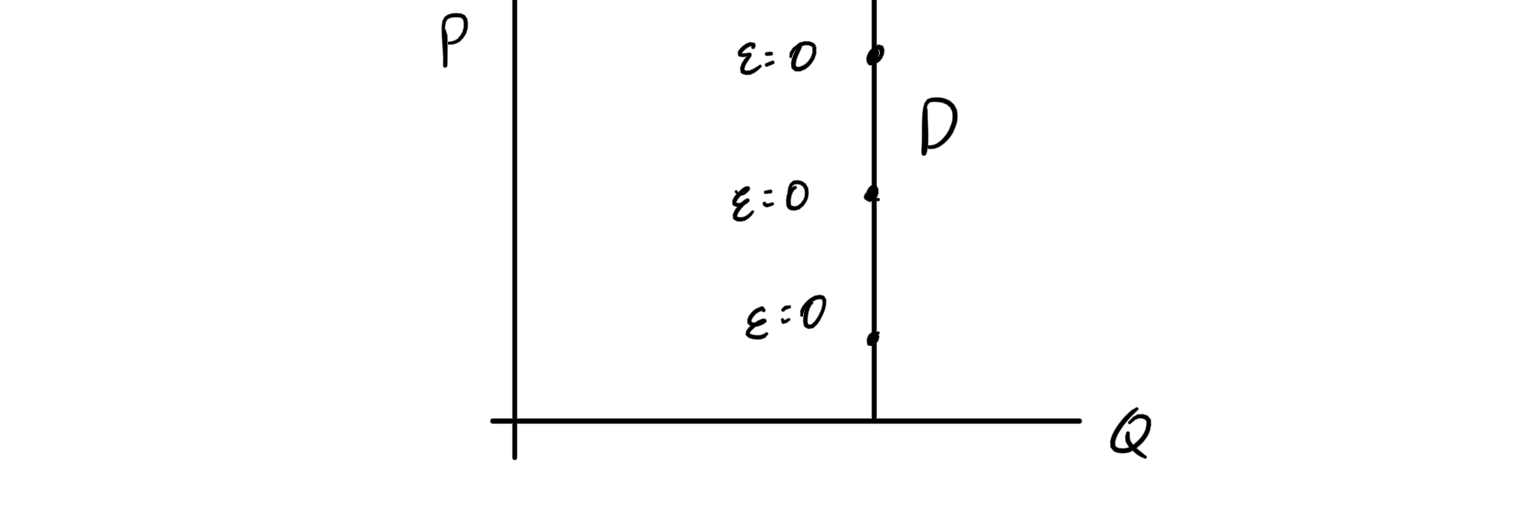
\includegraphics[scale=0.25]{img/Perfectly_Inelastic.PNG}
        \end{center}
        For example, insulin shots, despite their price, are needed regardless by people with diabetes. Therefore, an increase in the price of insulin shots will not change the need (i.e. the quantity demand) for these shots by the diabetics. 
      \end{definition}

      \begin{definition}[Price Elasticity of Supply]
        For a certain good $\mathfrak{g}$, its \textbf{elasticity of supply} refers to how sensitive the quantity supplied is to a change in its price. That is, 
        \begin{enumerate}
          \item If a price change of $\mathfrak{g}$ leads to a greater change in quantity supplied, then $\mathfrak{g}$ is said to be \textbf{elastic}. 
          \item If a price change of $\mathfrak{g}$ leads to a smaller change in quantity demanded, then $\mathfrak{g}$ is said to be \textbf{inelastic}. 
        \end{enumerate}
        Intuitively, it seems that 
        \[\frac{d q}{d p} = \frac{d (\text{quantity supplied})}{d (\text{price})}\]
        is the definition, but in actuality we measure the fractional response of $q$ to the fractional response of $p$. 
        \[\eta = \frac{\text{\% change in quantity } q}{\text{\% change in price } p}\]
        That is, 
        \[\eta = \frac{dq/q}{dp/p} = \frac{p}{S(p)} = \frac{p \, S^\prime (p)}{S(p)}\]
      \end{definition}

\section{Producer Theory}

  \begin{definition}[Firm as a Production Function]
    At the most basic level, a \textbf{firm} is an entity that transforms things into other, more valuable things, a process known as \textbf{production}. We can interpret the firm as a production function $f$ 
    \[f(\text{inputs}) = \text{output}\]
    Interpreting each input as $x_1, x_2, \ldots, x_n$ and output as $y$, we can model a firm buying $x_1$ amount of input 1, $x_2$ amount of input 2, ..., $x_n$ amount of input $n$ and producing an amount $y$ of the output. 
    \[f(x_1, x_2, \ldots, x_n) = y\]
    Ideally, firms would utilize a set of technologies for transforming things and then use this transformation to maximize net profits. 
  \end{definition}

  \begin{definition}[Types of Firms]
    There are 4 major types of firms created in law: 
    \begin{enumerate}
      \item A \textbf{proprietorship} is a firm owned by a single individual (the proprietor). The sole owner has \textit{unlimited liability} for the company and pays personal income taxes on profits earned. They are easy to establish and dismantle due to a lack in government regulations and requirements. 
      \item \textbf{Partnerships} share profits (equally or unequally). 
      \item A \textbf{corporation} is a legal entity that is separate and distinct from its owners. It offers \textit{limited liability}, meaning that shareholders may take part in the profits through dividends and stock appreciation but are not personally liable for the company's debts. However, it is costly (in money and time) to organize. Some types of corporations include: 
      \begin{enumerate}
        \item An \textbf{S corporation} (usually for smaller businesses with fewer than 100 shareholders) has the benefits of a corporation while being taxed as a partnership (i.e. no federal corporate taxes, only individual taxes). 
        \item A \textbf{limited liability corporation (LLC)} is a hybrid between a partnership and a corporation. They provide their owners with limited liability but like a partnership, LLCs' profits are taxed as part of the owners' personal income. 
      \end{enumerate}
      \item \textbf{Non-profit firms} is prohibited from distributing a profit to its owners. Religious operations, academic associations, environmental groups, hospitals, private universities are all organized as non-profit firms. They are not taxed by the government, given that they are engaged in government-approved activities. However, commercial profits (e.g. gift shops) are taxed. 
    \end{enumerate}
  \end{definition}

  \subsection{Production Functions}

    \begin{definition}[Cobb-Douglas Production Function]
      The \textbf{Cobb-Douglas production function} is one simple example model of a firm's production, defined 
      \[f(x_1, x_2, \ldots, x_n) = a_0 x_1^{a_1} x_2^{a_2} \ldots x_n^{a_n}\]
      The constants $a_1, a_2, \ldots, a_n$ are positive, generally less than $1$. For example, with two goods, capital $K$ and labor $L$, Cobb-Douglas can be expressed as 
      \[f(K, L) = a_0 K^a L_b\]
    \end{definition}

    \begin{definition}[Fixed-Proportions Production Function]
      The \textbf{fixed proportions} production function is defined
      \[f(x_1, x_2, \ldots, x_n) = \min \{a_1 x_1, a_2 x_2, \ldots, a_n x_n\}\]
      This function has the property that adding an input beyond a necessary level does no good. For example, the productive value of having more than one shovel per worker is quite low. 
    \end{definition}

    \begin{definition}[Inputs as Perfect Substitutes]
      Two inputs $K$ and $L$ are \textbf{perfect substitutes} in a production function $f$ is they enter as a sum. That is, if 
      \[f(K, L, \ldots, x_n) = g(K + c L, x_3, \ldots, x_n)\]
      for some constant $c$. In other words, with an appropriate scaling of the units of one of the variables, all that matters is the sum of the two variables, not the individual values. 
    \end{definition}

    \begin{definition}[Marginal Product]
      The \textbf{marginal product of an input} is just the partial derivative of the production function with respect to that input. That is, the marginal product of input $x_i$ is
      \[\frac{\partial f}{\partial x_i} \]
    \end{definition}

    \begin{example}[Marginal Product in Cobb-Douglas Function]
      In the two dimensional Cobb-Douglas production function with inputs $K$ and $L$ (and constant $A$):  
      \[f (K, L) = A K^\alpha L^\beta\]
      the marginal product of capital $K$ is 
      \[\frac{\partial f}{\partial K} (K, L) = \alpha A K^{\alpha-1} L^\beta\]
      Assuming that $0 < \alpha, \beta < 1$ (which is true in most cases), the marginal product of capital increases in the amount of labor, and decreases in the amount of capital. Indeed this is, since for example, an extra computer is very productive in a situation with lots of workers and few computers, but not so productive in a situation where there are lots of computers and few people to operate them. 

      The \textbf{value of the marginal product} of an input is basically just the marginal product times the price of the output. It is basically the value added by an additional unit of an input. If the value of the marginal product exceeds the cost of the input, then it is profitable to use more of that input. 
    \end{example}

    We now introduce the notions of short-term and long-term factors. 

    \begin{definition}
      Given the inputs $x_1, x_2, \ldots, x_n$ of a firm's production function, 
      \begin{enumerate}
        \item if an input $x_i$ can be adjusted (changed) quickly, it is called a \textbf{short-run factor}. Examples include cheap labor (McDonald's workers), simple equipment (shovels). 
        \item if an input $x_i$ can be adjusted (changed) slowly, it is called a \textbf{long-run factor}. Examples include very skilled labor (engineers) and expensive equipment (passenger aircraft).
      \end{enumerate}
    \end{definition}

  \subsection{Profit Maximization}

    \begin{definition}[Profit]
      Consider a production function 
      \[y = f(x_1, x_2, \ldots, x_n)\]
      where the marginal cost of renting/buying unit $x_i$ is $\omega_i$. Suppose $p$ is the price of the output $y$. Then, the \textbf{profit} $\pi$ is just the price of the total outputs minus the cost of renting/buying all the inputs, which can be represented by the function $\mathcal{C}$. That is, given inputs $x_1, x_2, \ldots, x_n$, the profit of the firm is:
      \[\pi = p \, f(x_1, \ldots, x_n) - \mathcal{C}(x_1, \ldots, x_n)\]
      However, in most cases the cost is expected to increase linearly with each input, giving the equation
      \[\pi = p \, f(x_1, \ldots, x_n) - \sum_{i=1}^n \omega_i x_i\]
      Using multivariate calculus, solving for when the Hessian matrix $H \pi$ is $0$ will find the vector $(x_1, \ldots, x_n)$ that maximizes $\pi$. 
    \end{definition}

    This function representation of firms gives us lots of flexibility in solving optimization problems. For example, given a firm with production function 
    \[f: \mathbb{R}^n \longrightarrow \mathbb{R}, \; y = f(x_1, x_2, \ldots, x_n)\]
    say that due to a lack of time, there is a limit on the amount of capital you can get that is constrained by the function 
    \[g(x_1, x_2, \ldots, x_n) \leq c\]
    for some constant $c$. (For example, you may have two inputs capital $K$ and labor $L$. It takes an hour to get additional capital and 2 hours to get additional labor. If you have 24 hours to get the capital, the constraint equation would be $K + 2L \leq 24$). Then $f$ can be easily optimized using the method of Lagrange multipliers (constrained to $c$). 

    \subsubsection{Shadow Value}

      \begin{definition}[Shadow Value]
        Given inputs $x_1, \ldots, x_n$, assume that the input $x_i$ for some $i$ in $1, \ldots, n$ cannot be adjusted on the short-run (e.g. a factory can't be built immediately). This creates a constraint on the profit available to the entrepreneur. Since $x_i$ is fixed, there is no direct value of $x_i$ because we can interpret the firm as a function without that one input; that is, as 
        \[f: \mathbb{R}^{n-1} \longrightarrow \mathbb{R}, \; f(x_1, \ldots, x_{i-1}, x_{i+1}, \ldots, x_n)\]
        But in the case that this constraint was relaxed (that is, if we could easily change the quantity of this input), we can measure its value. This is called the \textbf{shadow value}. That is, the shadow value of an input is the increase in profit associated with it. 
      \end{definition}

      \begin{example}[Shadow Value of Capital]
        Consider the capital/labor input firm. The profit of the firm is: 
        \[\pi = p F(K, L) - r K - \omega L\]
        Given a fixed capital $K_0$, let $L^*$ be the function of $K$ such that $L^*(K_0)$ is the value of labor that maximizes $\pi$. In other words, given a fixed value of capital $K = K_0$, the maximum value of $\pi$ is
        \[\pi\big(K_0, L^*(K_0)\big) = p F\big(K_0, L^*(K_0)\big) - r K_0 - \omega L^*(K_0)\]
        But assuming that we \textit{can} change this value (relaxing the constraint of $K = K_0$), we can view the above as a function of $K$. 
        \[\pi\big(K, L^*(K)\big) = p F\big(K, L^*(K)\big) - r K - \omega L^*(K)\]
        By taking the derivative of this with respect to $K$, we can see how a (hypothetical) change in $K$ will change the potential profit generated by the firm. The derivative below assumes that we can change $L$ accordingly.
        \[\frac{d \pi(K, L^* (K))}{d K} = p \frac{d F (K, L^*(K))}{d K} - r - \omega \frac{d L^*(K)}{dK}\]
        This ideal scenario where $L$ is changed accordingly can be shown by the hypothetical growth curve below: 
        \begin{center}
        %    \includegraphics[]{}
        \end{center}
        However, if $L$ cannot be changed accordingly, we can view the case as such: given that we are at fixed capital $K_0$ and optimized level of labor $L^*(K_0)$, we can calculate the shadow value of $K$ by keeping $L^*(K_0)$ constant while hypothetically changing $K$. Then we would relax the constraint $K=K_0$ (but not $L^* (K_0)$) 
        \[\frac{d \pi (K, L^* (K_0))}{dK} = \frac{d}{dK} \bigg( p F\big(K, L^*(K_0)\big) - r K - \omega L^*(K_0) \bigg) = p \frac{d F (K, L^*(K))}{d K} - r \]
        This in essence tells us the potential profit that can be generated by the firm by hypothetically increasing the capital \textit{with the current level of labor $L^*(K_0)$}. This scenario is shown by the straight line curve: 
        \begin{center}
        %    \includegraphics[]{}
        \end{center}
      \end{example}

      Over the long run, the firm can adjust both the capital and the labor. That is, let $L^{**}$ and $K^{**}$ be the labor and capital, respectively, that maximizes the profit $\pi$. This can be found using regular optimization methods in multivariate calculus. 

      \begin{example}[Cobb-Douglas]
        The Cobb-Douglas production function has profit
        \begin{align*}
            \pi & = p F(K, L) - r K - \omega L \\
            & = p A K^\alpha L^\beta - r K - \omega L
        \end{align*}
        Optimizing $\pi$ gives the solutions 
        \[L^{**} = \Bigg(\frac{A p \alpha^\alpha \beta^{1-\alpha}}{r^\alpha \omega^{1-\alpha}} \Bigg)^{\frac{1}{1-\alpha-\beta}}, \text{ and } K^{**} = \Bigg(\frac{A p \alpha^{1-\beta} \beta^\beta}{r^{1-\beta} \omega^\beta}\Bigg)^{\frac{1}{1-\alpha-\beta}} \]
        While these solutions may appear complicated, they make sense. They are proportionally dependent on the output price $p$, and the input prices $r$ and $\omega$ shows straightforward relationships too. 
      \end{example}

    \subsubsection{Types of Costs}

      We define 5 types of cost functions. 

      \begin{definition}[Short-Run Total Cost]
        Suppose that given a firm's production function $f$ with inputs $x_1, x_2, \ldots, x_n$ and output $y$, with $\mathcal{C}$ the cost function such that
        \[\pi = f - \mathcal{C}\]
        Now, assume that you want to produce at least quantity $q$ of the output. Then, the \textbf{short-run total cost of producing $q$} is
        \[\SRTC(q) \equiv \min_{x_1, \ldots, x_n} \{ \mathcal{C}(x_1, \ldots, x_n) \;|\; F(x_1, \ldots, x_n) \geq q\}\]
        In other words, it is the minimum cost of producing at least $q$ outputs. Furthermore, we can account for units that are not adjustable in the short run. Suppose there are $k$ inputs $x_{j_1}, \ldots, x_{j_k}$ that are not adjustable in the short-run. Then, the \textbf{short-run total cost of producing $q$, given the quantity $x_{j_1} = x_{j_1}^*, \ldots, x_{j_k} = x_{j_k}^*$}, is 
        \begin{align*}
            \SRTC(q\,|\, x_{j_i} = x_{j_i}^* \;\forall\; i = 1, \ldots, k) = \min_{x} \{ \mathcal{C}(x) \;|\; F(x) \geq q, x_{j_i} = x_{j_i}^* \;\forall\; i = 1, \ldots, k\}
        \end{align*}
        where $x$ represents the vector $(x_1, \ldots, x_n)$. 
        More simply put, $\SRTC(q\,|\, x_i)$ is merely just $\SRTC(q)$ restricted to the level set formed by the intersections of the $k$ hyperplanes $x_{j_1} = x_{j_1}^*, \ldots,  x_{j_k} = x_{j_k}^*$. 
      \end{definition}

      \begin{definition}[Short-Run Marginal Cost]
        The \textbf{short-run marginal cost of producing $q$} is just the derivative of $\SRTC(q)$. 
        \[\SRMC(q) = \frac{d}{dq} \SRTC(q) = \SRTC^\prime (q)\]
        That is, it is the additional cost incurred if we were to produce one more unit of the output ($q+1$ outputs). Similarly, the \textbf{short-run marginal cost of producing $q$, given the quantity $x_i = x_{i0}$}, is 
        \[\SRMC(q\,|\, x_{j_i} = x_{j_i}^* \;\forall\; i = 1, \ldots, k) = \SRTC^\prime (q\,|\, x_{j_i} = x_{j_i}^* \;\forall\; i = 1, \ldots, k)\]
        It is the additional cost incurred if we were to produce one more unit of the output, given that we cannot change input $x_i = x_{i0}$. 
      \end{definition}

      \begin{definition}[Short-Run Average Cost]
        The \textbf{short run average cost of producing $q$} is simply obtained by dividing the short-run total cost by the quantity produced. 
        \[\SRAC (q) = \frac{\SRTC(q)}{q}\]
        As the name suggests, it is the average (minimum) cost of producing quantity $q$ outputs. If we are restricted in input $x_i = x_{i0}$, then 
        \[\SRAC(q\,|\, x_{j_i} = x_{j_i}^* \;\forall\; i = 1, \ldots, k) = \frac{\SRTC^\prime (q\,|\, x_{j_i} = x_{j_i}^* \;\forall\; i = 1, \ldots, k)}{q}\]
      \end{definition}

      \begin{definition}[Short-Run Average Variable Cost]
        Assume that we have a fixed costs of operations 
        \[x_{j_1} = x_{j_1}^*, x_{j_2} = x_{j_2}^*, \ldots, x_{j_k} = x_{j_k}^*\] 
        Then, the \textbf{short-run average variable cost of producing $q$} eliminates the fixed costs of operation to get the average short-run cost. For simplicity of notation, we will shorten 
        \[\big( x_{j_i} = x_{j_i}^* \;\forall\; i \in [1,k]\big) \implies \big(  x_{j_i} = x_{j_i}^*  \big)\]
        and assume that there are $k$ restricted costs. Then, we have 
        \[\SRAVC(q\,|\, x_{j_i} = x_{j_i}^*) = \frac{\SRTC(q\,|\, x_{j_i} = x_{j_i}^*) - \SRTC(0\,|\, x_{j_i} = x_{j_i}^*)}{q}\]
        We can just imagine $\SRAVC(q)$ as calculating the short-run average cost, given that an external party paid for all fixed costs of operations. This means that if there are no fixed costs, then 
        \[\SRAVC = \SRAC\]
      \end{definition}

      \begin{example}
        Given a firm production function $F$ with inputs capital $K$ and labor $L$, let capital $K$ be non-adjustable on the short run, set at $K=k$ and let the cost function be
        \[\mathcal{C}(K, L) = r K + \omega L\]
        In order to find the $\SRTC(q)$, we must minimize $\mathcal{C}$, so the constraint $F(K, L) \geq q$ is really satisfied with equality $F(K, L) = q$. But since $K=k$ is a constant, the equation
        \[F(k, L) = q\]
        which maps $l \mapsto F(k, l) = q$, also determines a mapping from $q$ to $L$ by the implicit function theorem. We will call this function $L_S$, defined such that
        \[F\big( k, L_S (q)\big) = q\]
        The short run total cost of producing $q$, given $K=k$, is 
        \[\SRTC(q\,|\,K=k) = r k + \omega L_S (q)\]
        The implicit function theorem also states that since $F(k, \cdot)$ and $L_S (\cdot)$ are inverses, 
        \[\frac{d L_S (q)}{d q} \bigg|_{F = q} = \frac{1}{\frac{\partial F}{\partial L} \big(k, L_S (q)\big)}\]
        Therefore, 
        \[\SRMC(q\,|\,K=k) = \SRTC^\prime (q\,|\,K=k) = \frac{d}{dq} (r k + \omega L) = \omega \frac{d L}{d q} \bigg|_{F=q} = \frac{\omega}{\frac{\partial F}{\partial L} \big(k, L_S (q)\big)}\]
        Then, 
        \[\SRAC(q\,|\,K=k) = \frac{\omega}{q \frac{\partial F}{\partial L} \big(k, L_S (q)\big)}\]
        Finally, 
        \[\SRAVC(q\,|\,K=k) = \frac{\SRTC(q\,|\,K=k) - \SRTC(0\,|\,K=k)}{q} = \frac{\omega L_S (q\,K=k)}{q}\]
      \end{example}

      \begin{definition}[Long-Run Total Cost]
        On the long run, all inputs can vary, meaning that the long-run cost doesn't need to be conditioned on the $x_{j_i}$'s. Therefore, \textbf{long-run total cost of producing $q$} is 
        \[\LRTC (q) = \min_{x} \{\mathcal{C}(x)\;|\; F(x) \geq q\}\]
      \end{definition}

      \begin{definition}[Long-Run Marginal Cost]
        The \textbf{long run marginal cost of producing $q$} is the derivative of the long run total cost. 
        \[\LRMC (q) = \LRTC^\prime (q)\]
      \end{definition}

      \begin{definition}[Long-Run Average Cost]
        The \textbf{long-run average cost} is 
        \[\LRAC (q) = \frac{\LRTC(q)}{q} \]
        It is clear that since all costs are variable, we don't have to deal with constraints and therefore the $\LRAC$ is the same as the long run average variable cost. 
      \end{definition}

      \begin{example}[Cobb-Douglas]
        For the Cobb-Douglas production function $F(K, L) = A K^\alpha L^\beta$, with $\alpha + \beta < 1$, with $K=k$ fixed in the short-run but not on the long run, we have
        \begin{align*}
          \SRTC(q\,|\,K=k) & = r K + \omega \bigg(\frac{q}{A K^\alpha} \bigg)^{\frac{1}{\beta}} \\
          \SRAVC(q\,|\,K=k) & = \omega \frac{q^{(1-\beta)/\beta}}{(A K^\alpha)^{1/\beta}} \\
          \SRMC(q\,|\,K=k) & = \omega \frac{q^{(1 - \beta)}}{\beta}{\beta (A K^\alpha)^{1/\beta}} \\
          \LRTC(q\,|\,K=k) & = \Bigg( \Big(\frac{\alpha}{\beta}\Big)^{\frac{\beta}{\alpha + \beta}} + \Big(\frac{\beta}{\alpha}\Big)^{\frac{\alpha}{\alpha + \beta}} \Bigg) \omega^{\frac{\beta}{\alpha + \beta}} r^{\frac{\alpha}{\alpha + \beta}} \bigg(\frac{q}{A}\bigg)^{\frac{1}{\alpha + \beta}}
        \end{align*}
      \end{example}

    \subsubsection{Dynamic Firm Behavior}

      We will describe how a firm that produces output $y$ responds to price changes of $y$. Assume that the price of a unit of $y$ is $p$. Then, the firm earns profits 
      \[\pi = p q - \mathcal{C}(q\,|\,K = k)\]
      where $\mathcal{C}(q\,|\,K=k)$ is the total cost of producing given that the firm currently has capital $k$. To maximize profits, the firm chooses quantity $q_s$ such that 
      \[0 = p - \mathcal{C}^\prime (q\,|\,K = k) \implies p = \mathcal{C}^\prime (q\,|\,K = k)\]
      i.e. when the price equals marginal cost. Obviously, this is a good strategy only if producing a positive quantity is desirable, that is, if 
      \[p q_s - \mathcal{C}(q_s\,|\,K=k) \geq p \cdot 0 - \mathcal{C} (0\,|\,K=k)\] 
      This can be written as
      \[p \geq \frac{\mathcal{C}(q_s \,|\, K=k) - \mathcal{C}(0, K=k)}{q_s} = \SRAVC(q_s\,|\,K=k)\]
      This means that the firm will start producing products provided that its price exceeds the average variable cost. 

      \begin{theorem}
        The profit maximizing firm produces the quantity $q_s$ where price equals marginal cost, provided price is as large as minimum average variables cost. If price falls below the minimum average variable cost, the firm shuts down. 
      \end{theorem}

      Let us draw the supply curve of the firm; that is, the curve that represents the choice of the firm (on the quantity it supplies) as a function of the price (the thick line).
      \begin{center}
      %    \includegraphics[]{}
      \end{center}
      Therefore, if the price is above the minimum average variable cost (AVC), the firm shuts down since the average revenue (not accounting for fixed costs) it makes on producing is less than the marginal cost. When price is above the minimum average variable cost, the marginal cost gives the quantity supplied by the firm. 

      We can also talk about the average total cost, 

  \subsection{Perfect Competition Dynamics}

  \subsection{Investment}

    \begin{definition}[Time Value of Money]
      The promise of \$1 in the future is not worth \$1 today, since having the \$1 right now allows us to invest it immediately to get returns. The \textbf{present value} of a dollar is worth more than the \textbf{discounted value} of a dollar in the future. 

      The interest rate of U.S. Treasury bonds (which are the most secure investment) allows us to determine the potential rate of return of \$1 if we were to invest it. That is, if we have $\mathcal{X}$ amount of dollars and the interest rate is $r$, then in one year we are guaranteed 
      \[\mathcal{X} \cdot (1 + r)\]
      dollars. That means that $\mathcal{X}$ dollars in the present value is worth $\mathcal{X}(1 + r)$ dollars in the future value. Going backwards, if we are guaranteed $\mathcal{Y}$ dollars a year in the future, then the present value of it is
      \[\frac{\mathcal{Y}}{1 + r}\]
      The present value PV has a simple formula. Say that $r_1$ is the interest rates this year, $r_2$ interest rates next year, and so on. If we obtain a stream of payments $A_0$ immediately, $A_1$ at the end of year 1, $A_2$ at the end of year 2, and so on, the present value of the stream of payments is
      \[\text{PV} = A_0 + \frac{A_1}{1 + r_1} + \frac{A_2}{(1+r_1) (1+r_2)} + \frac{A_3}{(1+r_1) (1+r_2) (1+r_3)} + \ldots\]
      All financial analyses that assumes this concept of discounted future value of money is called \textbf{DCF (Discounted Cash Flow) analysis}.
    \end{definition}

    \begin{example}
      For example, given that \$10,000 is invested for one year at 10\% interest, the future value of that money is: 
      \[FV = \$10,000 \times \bigg(1 + \frac{10\%}{1}\bigg)^{1 \times 1} = \$11,000\]
      This means that \$10,000 now is equal to \$11,000 in the future. The value of \$5,000 one year from today, compounded at 7\% interest, is: 
      \[PV = \$5,000 \bigg/ \bigg(1 + \frac{7\%}{1}\bigg)^{1 \times 1} =  \$4,673\]
      If we increase the rate of compounding, it can change future values: 
      \begin{enumerate}
          \item Quarterly Compounding: $FV = \$10,000 \times \Big( 1 + \frac{10\%}{4}\Big)^{4 \times 1} = \$11,038$
          \item Monthly Compounding: $FV = \$10,000 \times \Big( 1 + \frac{10\%}{12}\Big)^{12 \times 1} = \$11,047$
          \item Daily Compounding: $FV = \$10,000 \times \Big( 1 + \frac{10\%}{365}\Big)^{365 \times 1} = \$11,052$
      \end{enumerate}
      This means that TVM depends not only on interest rate and time horizon, but also no how many times the compounding calculations are computed each year. 
    \end{example}

    \begin{definition}[Consols]
      Bonds that pay a fixed amount every year \textit{forever} are known as \textbf{consolidated annuities}, or \textbf{consols}. The value $v$ of a consol that pays a fixed $A$ dollars every year in an economy with a fixed interest rate $r$ is 
      \[v = \frac{1}{1+r} + \frac{1}{(1+r)^2} + \frac{1}{(1+r)^3} + \ldots  = \frac{1}{1 - \frac{1}{1+r}} - 1 = \frac{1}{r}\]
      Note that as interest rates decrease, consols become more valuable. For example, at a 5\% interest rate, \$1 million paid per year will be worth \$20 million today. 
    \end{definition}

    \begin{example}[Mortgages]
      We now fix a monthly interest rate $r$. We will treat a mortgage as a fixed payment per month for a large number of months (e.g. 360 months for a 30 year mortgage). The present value of these payments over $n$ months is 
      \[M = \frac{1}{1+r} + \frac{1}{(1+r)^2} + \ldots + \frac{1}{(1+r)^n} = \frac{1}{r} \bigg( 1 - \frac{1}{(1+r)^n}\bigg)\]
      To put this into perspective, at a monthly interest rate of 0.5\%, paying \$1 per month for 360 months produces a present value $M$ of \$166.79. 
      \[M = PV = \frac{1}{1.005} + \frac{1}{1.005^2} + \ldots + \frac{1}{1.005^360} \approx 166.79\]
      Since \$1 per month for 360 months generates \$166.79 in present value, scaling this up, we can see that \$599.55 per month for 360 months generates \$100,000 in present value. Therefore, to get a current loan of \$100,000, you will be expected to pay back \$599.55 per month for the next 360 months in order to pay back the present value's worth. 
    \end{example}

    \begin{example}
      \$20,000,000 paid right now to you is great. Now, assume that you are paid \$1,000,000 per year for the next 20 years, with the first payment happening immediately. With the interest rate being $r$, the present value of the \$20 million would be
      \[\text{PV} = 1000000 + \frac{1000000}{1 + r} + \frac{1000000}{(1+r)^2} + \ldots + \frac{1000000}{(1+r)^{19}}\]
      The table below shows what the present value (in thousands) would be at various interest rates: 
      \begin{center}
      \begin{tabular}{c|c|c|c|c|c|c}
          r &  3\% & 4\% & 5\% & 6\% & 7\% & 10\%\\
          \hline
          PV & \$15,324 & \$14,134 & \$13,085 & \$12,158 & \$11,336 & \$9,365
      \end{tabular}
      \end{center}
      It is clear that interest rates can make a dramatic impact on future value. Cutting them by 25\% or even more than 50\% in some interest rates. 
    \end{example}

    From looking at a Treasury bill (which offers a one-time payment after $n$ years), we can also calculate the effective interest rate $r$. For example, say that a $n$-year bond that will pay \$10,000 is sold at \$9,615.39. We can see that this produces a 4\% interest rate by solving the equation
    \[10,000 \cdot (1 + r)^n = 9,615\]
    for $r$. In general, let the price of the bill be $P$ and its future value (the amount it will pay when the bill matures) is FV. Then
    \[P\cdot (1 + r)^n = \text{FV} \implies r = \bigg( \frac{FV}{P} \bigg)^{1/n} - 1\]

    \begin{definition}[Net Present Value of Bonds]
      Bonds are generally collected semi-annually, but they have a fixed interest rate set at the time of issue during the life of the bond. A $n$-year \$$\mathcal{X}$ bond at interest rate $r$ with semi-annual payments would have a \textbf{net present value} (i.e. how much it is worth now in present value) of 
      \[\text{NPV} = \frac{nr/2}{(1+r)^{\frac{1}{2}}} + \frac{nr/2}{(1+r)^{1}} + \frac{nr/2}{(1+r)^{\frac{3}{2}}} + \ldots + \frac{nr/2}{(1+r)^{\frac{2n-1}{2}}} + \frac{nr/2}{(1+r)^{n}} + \frac{n}{(1+r)^{n}}\]
      For example, a three-year \$10,000 bond at 5\% with semi-annual payments would pay \$250 at the end of every half-year for every 3 years, and pay \$10,000 at the end of the three years. The NPV of this bond, with annual interest $r$ (determined by the economy), would be
      \[\text{NPV} = \frac{\$250}{(1+r)^{\frac{1}{2}}} + \frac{\$250}{(1+r)^{1}} + \frac{\$250}{(1+r)^{\frac{3}{2}}} + \frac{\$250}{(1+r)^{2}} + \frac{\$250}{(1+r)^{\frac{5}{2}}} + 
      \frac{\$250}{(1+r)^{3}} + \frac{\$10,000}{(1+r)^{3}}\]
      The NPV would be the price of the bond. So, it is important to remember that a bond loses value when interest rates rise. This is because with a rise in interest rates, more attractive bonds with better coupon payments are produced. Therefore, it is good to buy bonds when interest rates are high. When the interest rates drop afterwards, the value of the bond becomes even higher. 
    \end{definition}

    \subsubsection{Corporate Investment}

      \begin{definition}[NPV Analysis]
        Consider an investment project involving spending an investment $I$ and then reaping a return over time. We can represent the \textbf{net present value} of this investment as 
        \[\text{NPV} = -I + \frac{R_1}{1+r} + \frac{R_2}{(1+r)^2} + \frac{R_3}{(1+r)^3} + \ldots\]
        where $R_1$ represents first year revenues, $R_2$ represents second year revenues, and so on. The investment is made when NPV is positive. A NPV analysis requires three things:
        \begin{enumerate}
          \item Initial investment $I$ must be estimated
          \item Revenues $R_1, R_2, \ldots$ must be estimated, which can be heard since new products (new tech) or uncertain outcomes (e.g. oil wells) provide no way of estimating demand
          \item An appropriate rate of return $r$, which is the discount rate that represents the return that could be earned per year on an investment of similar risk
        \end{enumerate}
        Note that this analysis could be subject to bias, since project leaders would try to minimize $I$, maximize the $R_i$'s, and minimize $r$ in order to make the project look more attractive to upper management. 
      \end{definition}

      \begin{example}[Silver Mine]
        A company looking to develop a silver mine in Mexico estimates that developing the mine would require \$4 million per year for four years, Then, it generates a revenue of \$1 million per year for 40 years. Then, the net present value (in millions) is 
        \[\text{NPV} = -4 + \frac{-4}{1.18} + \frac{-4}{1.18^2} + \frac{-4}{1.18^3} + \frac{1}{1.18^4} + \ldots + \frac{1}{1.18^{43}} = -12.697 + 13.377 = 0.81\]
        This leads to a revenue of \$810,000. In actuality, the problem with mines is that an 18\% rate of return makes those future revenues have quite modest present values. 
      \end{example}

      \begin{definition}[Internal Rate of Return Analysis]
        Similar to NPV analysis, the IRR analysis solves the equation
        \[\text{NPV} = 0\]
        for the interest rate $r$, and then the project is undertaken if the rate of return is sufficiently high. However, this equation may have more than one solution or no solutions at all, so it is not transparent what to do in these events. 
      \end{definition}

      \begin{definition}[Payback Method]
        The payback method asks how many years a project must be run before profitability is reached. That is, it solves the equation
        \[\text{NPV} = 0\]
        for the number of years $n$. 
      \end{definition}

      Note that the NPV approach does a good job when the question is whether to undertake a project or not (better than most approaches in investment decisions), making it the most common approach to investment decisions. However, NPV does a poor job when the question is whether to undertake a project or to delay the project. 

    \subsubsection{Option Value of Investment}

      We now deal with the question of whether to undertake an investment project or delay it. When we invest in some products, like oil, the value of this investment can \textit{change} over time. This change leads to \textit{price risk}, which NPV analysis has a hard time predicting. 

      Say that there is a good $\mathfrak{g}$ that you have spent a constant cost $\mathcal{C}$ investing in (e.g. you've spent \$50 on a stock). To normalize this, assume that $0 < \mathcal{C} < 1$. As soon as $\mathcal{C}$ is invested, a value $\mathcal{V}$ is generated, but it varies from time to time in a random manner. Say that the distribution in value (again, normalized) is
      \[\mathcal{V} \sim \text{Uniform}[0,1] \implies \mathbb{P}(V \in [a,b]) = |b-a|\]
      We can set a \textbf{cutoff value} $V_0$: that is, set a level $V_0$ and invest in the option if and only if $\mathcal{V} \geq V_0$. The NPV rule simply says $V_0 = C$; that is, invest whenever profitable. 

      Now, given that we have invested $\mathcal{C}$ into the option (with value represented by the random variable $\mathcal{V}$) with cutoff value $V_0$, let us model this as a discrete time Markov chain with initial distribution to be at node $A$ with probability $V_0$ and node $B$ with probability $1-V_0$. 
      \begin{center}
        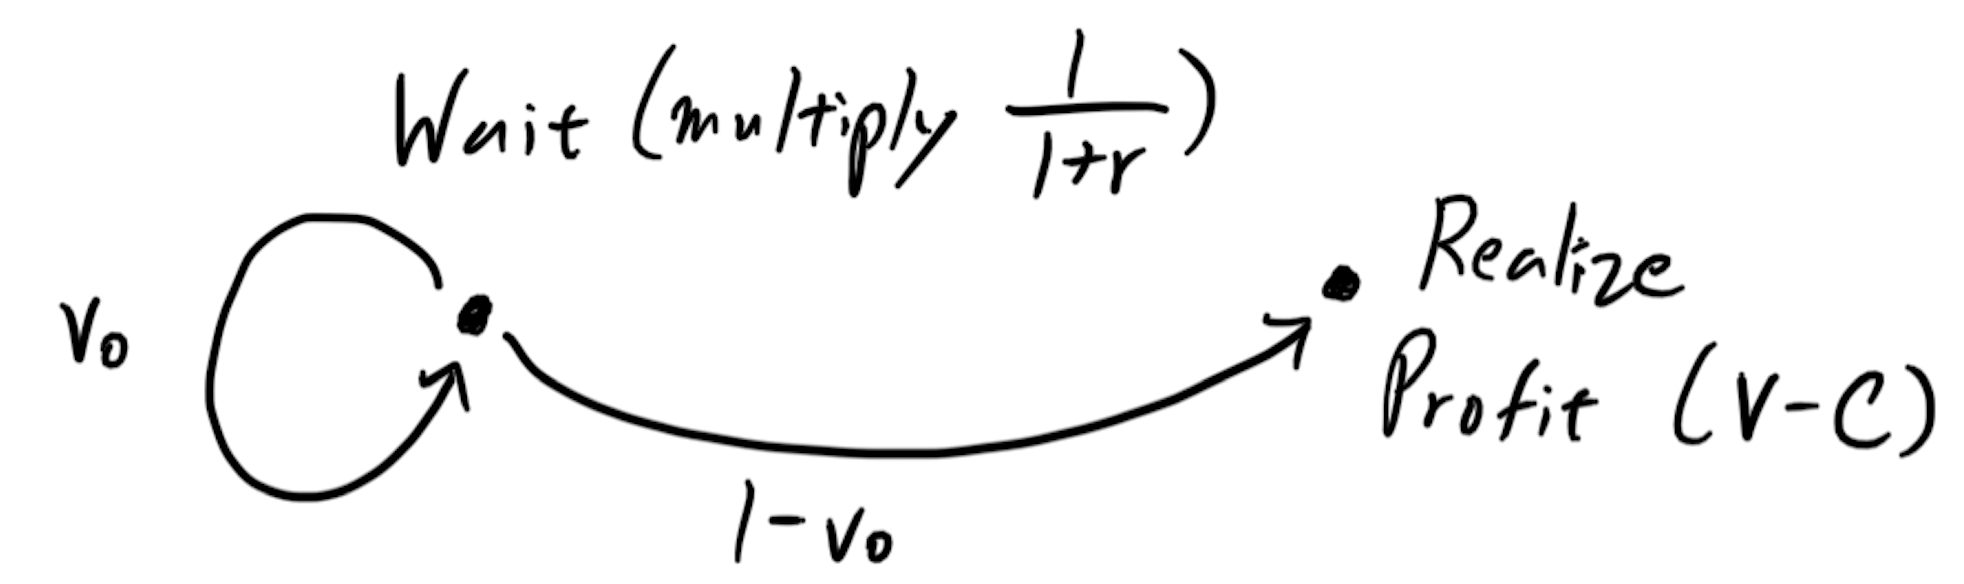
\includegraphics[scale=0.25]{img/Option_Investment_Graph.PNG}
      \end{center}
      To elaborate, landing on node $A$ will require us to wait another year to realize the investment, requiring us to discount the value of $\mathfrak{g}$ by $\frac{1}{1+r}$. But when we land on node $B$ (the absorbing state), the investment is automatically realized and we take profit (not discounted yet) defined by random variable
      \[\big( \mathcal{V} - \mathcal{C} \;|\; \mathcal{V} \in [V_0, 1]\big) \sim \text{Uniform}[V_0 - \mathcal{C}, 1 - \mathcal{C}]\]
      However, to make things simpler, we can just compute the expectation of profit (not discounted yet) upon landing on node $B$. By linearity,
      \[\mathbb{E} \big( \mathcal{V} - \mathcal{C} \;|\; \mathcal{V} \in [V_0, 1]\big) = \frac{1 + V_0}{2} - \mathcal{C}\]
      Since the number of times $k$ that the chain lands on node $A$ before landing on node $B$ (the absorbing state) is a random variable, the discounted profit $J$ behaves like a geometric random variable: 
      \[\mathbb{P} \Bigg( J = \bigg(\frac{1}{1+r}\bigg)^k \bigg(\frac{1 + V_0}{2} - \mathcal{C} \bigg) \Bigg) = V_0^k \big( 1-V_0\big)\]
      The expectation of profit $J$ can be found by conditioning on $k$: 
      \[\mathbb{E}(J) = \sum_{k = 0}^\infty \bigg(\frac{1}{1+r}\bigg)^k \bigg( \frac{1 + V_0}{2} - \mathcal{C}\bigg) V_0^k \big(1 - V_0\big) = \cfrac{\big(1 - V_0\big) \Big(\cfrac{1+V_0}{2} - \mathcal{C}\Big)}{1 - \cfrac{V_0}{1+r}}\]
      We can actually treat this as a function of the cutoff value $V_0$ to get 
      \[( \mathbb{E} J)(V_0) = \cfrac{\big(1 - V_0\big) \Big(\cfrac{1+V_0}{2} - \mathcal{C}\Big)}{1 - \cfrac{V_0}{1+r}}\]
      Therefore, given that we have a cutoff value $V_0$, $(\mathbb{E} J) (V_0)$ tells us the firm's expected profit given this $V_0$. We can get a clue as to what this function looks like. Differentiating it with respect to $V_0$ gives 
      \[( \mathbb{E} J)^\prime (V_0) = \cfrac{1 + 2r \mathcal{C} + V_0^2 - 2(1+r) V_0}{2 (1+r) \bigg( 1 - \frac{V_0}{1+r}\bigg)^2}\]  
      which implies that $(\mathbb{E} J)^\prime (\mathcal{C}) > 0$ and $(\mathbb{E}J)^\prime (1) < 0$. This means that there is a maximum at $(C, 1)$, which is calculated to be
      \[V_0 = (1 + r) \pm \sqrt{r^2 + 2r (1-\mathcal{C})}\]
      The positive root of the quadratic has $V_0 > 1$, which entails never investing. Therefore, the profit maximizing investment strategy is to invest whenever the value $\mathcal{V}$ exceeds 
      \[V_0 = (1 + r) - \sqrt{r^2 + 2r (1-\mathcal{C})}\]
      Two things to note: 
      \begin{enumerate}
        \item When $r=0$, then $V_0 = 1$. This makes sense because $r=0$ corresponds to no discounting, so there is no loss in holding out for the highest possible value. 
        \item As $r \rightarrow \infty$, $V_0 \rightarrow \mathcal{C}$. $r \rightarrow \infty$ means that the future is valueless, so it is worth investing if the return is anything over its costs. Therefore, the NPV rule only applies if the future is valueless. 
      \end{enumerate}
      We can present the deviation of this option value analysis with NPV analysis. That is, given the cost $\mathcal{C}$, the different curves represent $\mathbb{E} J$ as a function of the interest rate $r$. 
      \begin{center}
      %    \includegraphics[]{}
      \end{center}
      Note that as $r = 0$, it doesn't matter what the cost is; the cutoff value when we should realize the investment is at $V_0 = 1$, since we can keep waiting. But looking at each case individually, 
      \begin{enumerate}
        \item For the curve representing $\mathcal{C} = 0$, as the interest rate $r$ increases the future value of the investment gets diminished quickly and so the cutoff value $V_0 = \mathbb{E} J$ will likewise decrease. 
        \item For $\mathcal{C} = 0.25$, there is an additional cost incurred, meaning that we must have an additional profit, that is, a higher cutoff value $V_0$, than $\mathcal{C} = 0$, given the same interest rate. 
        \item Following this line of thought, $\mathcal{C} = 0.5$ will have an higher cutoff value $V_0$ than that of $\mathcal{C} = 0.25$. 
      \end{enumerate}
      We can draw three additional curves that represent the cutoff value according to NPV analysis: $V_0 = \mathcal{C}$. 
      \begin{center}
      %    \includegraphics[]{}
      \end{center}
      We can see that the optimal strategy deviates significantly from the NPV strategy. 

    \subsubsection{Resource Extraction and Harvest}

      \begin{example}
        Suppose that you believe that the world will run out of oil, so you invest in it by buying it and holding it. If you buy a barrel at \$40 and sell it for \$1000 in 20 years, you get a profit of \$960. 

        We can interpret this profit in terms of interest rates. More specifically, the \textbf{Ramsey rule} implies that the prices of resources that are in fixed supply rise at the interest rate. Therefore, we can view this profit as a constant interest rate that accumulates on the price of oil for 20 years: 
        \[\$40 \, (1 + r)^{20} = \$1000 \implies r = 17.46\%\]
      \end{example}

      We formulate this mathematically. 

      \begin{example}
        Let time run in discrete intervals $t = 0, 1, \ldots$ and suppose that the demand for a resource in fixed supply has constant elasticity: 
        \[p(Q) = a Q^{\frac{1}{\varepsilon}}\]
        Suppose that there is a total stock $R$ of the resource with interest rate fixed at $r$. Let's find the price and consumption of the resource at each time. 

        Letting $Q_t$ represent the quantity consumed at time $t$, we can see that discounting future prices gives us 
        \[p(Q_0) (1 + r)^t = p(Q_t)\]
        so
        \[a Q_0^{-1/\varepsilon} (1 + r)^t = p (Q_0) (1+r)^t = p(Q_t) = a Q_t^{-1/\varepsilon} \implies Q_t = Q_0 (1+r)^{- t \varepsilon}\]
        Finally, the resource constraint implies that 
        \[R = \sum_{i=0}^\infty Q_i = Q_0 \sum_{i=0}^\infty (1+r)^{-i \varepsilon} = \frac{Q_0}{1 - (1+r)^{-\varepsilon}}\]
        This solves 
        \begin{align*}
          Q_0 & = R \big( 1 - (1+r)^{-\varepsilon}\big) \\
          Q_1 & = Q_0 (1 + r)^{\varepsilon}\\
          Q_2 & = \ldots
        \end{align*}
        To represent this graphically, we can see below: 
        \begin{center}
          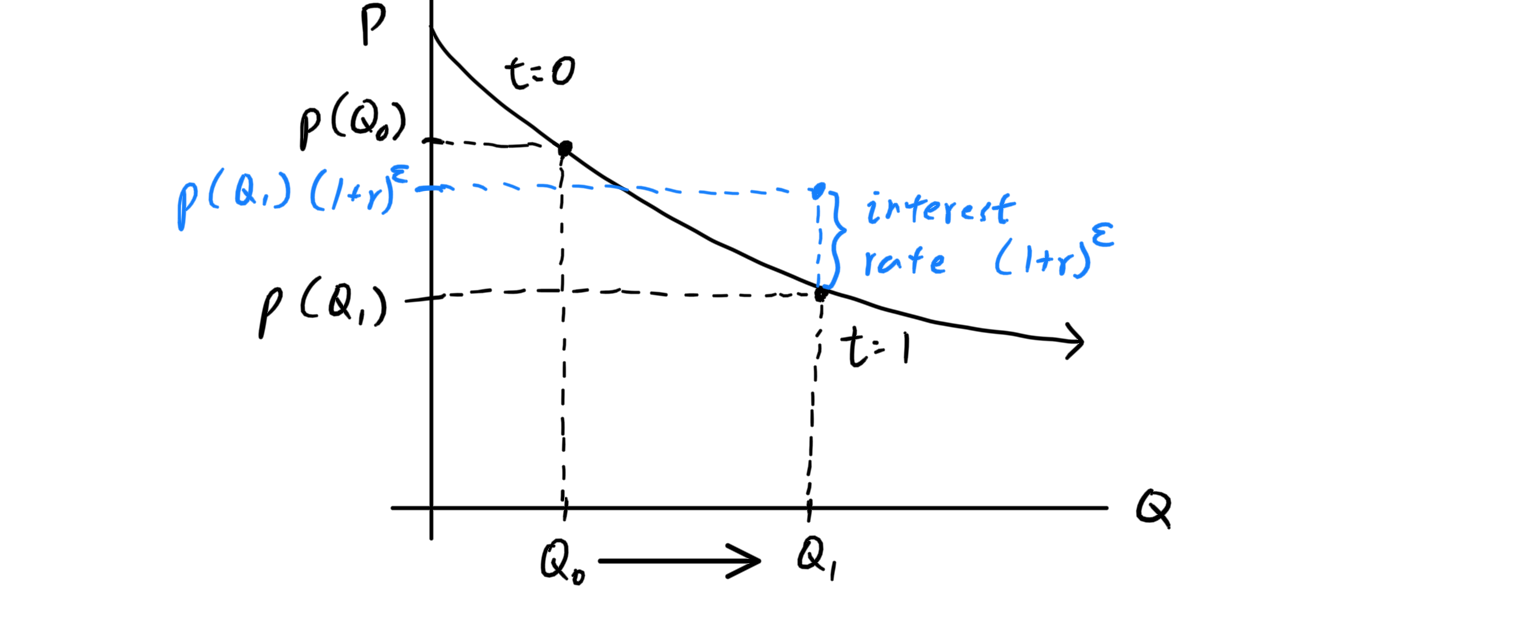
\includegraphics[scale=0.25]{img/Demand_Curve_Constrained_Resource.PNG}
        \end{center}
      \end{example}

\end{document}
